\documentclass[12pt,]{article}
\usepackage{lmodern}
\usepackage{amssymb,amsmath}
\usepackage{ifxetex,ifluatex}
\usepackage{fixltx2e} % provides \textsubscript
\ifnum 0\ifxetex 1\fi\ifluatex 1\fi=0 % if pdftex
  \usepackage[T1]{fontenc}
  \usepackage[utf8]{inputenc}
\else % if luatex or xelatex
  \ifxetex
    %\usepackage{mathspec}
    \usepackage{unicode-math}
    \usepackage{xltxtra,xunicode}
  \else
    \usepackage{fontspec}
  \fi
  \defaultfontfeatures{Mapping=tex-text,Scale=MatchLowercase}
  \newcommand{\euro}{€}
    \setmainfont{TeX Gyre Pagella}
\fi
% use upquote if available, for straight quotes in verbatim environments
\IfFileExists{upquote.sty}{\usepackage{upquote}}{}
% use microtype if available
\IfFileExists{microtype.sty}{%
\usepackage{microtype}
\UseMicrotypeSet[protrusion]{basicmath} % disable protrusion for tt fonts
}{}
\usepackage[left=2.5cm,right=2.5cm,top=2.5cm,bottom=2.5cm]{geometry}
\ifxetex
  \usepackage[setpagesize=false, % page size defined by xetex
              unicode=false, % unicode breaks when used with xetex
              xetex]{hyperref}
\else
  \usepackage[unicode=true]{hyperref}
\fi
\hypersetup{breaklinks=true,
            bookmarks=true,
            pdfauthor={Gavin L. Simpson},
            pdftitle={Modelling palaeoecological time series using generalized additive models},
            colorlinks=true,
            citecolor=blue,
            urlcolor=blue,
            linkcolor=magenta,
            pdfborder={0 0 0}}
\urlstyle{same}  % don't use monospace font for urls
\setlength{\parindent}{0pt}
\setlength{\parskip}{6pt plus 2pt minus 1pt}
\setlength{\emergencystretch}{3em}  % prevent overfull lines
\providecommand{\tightlist}{%
  \setlength{\itemsep}{0pt}\setlength{\parskip}{0pt}}
\setcounter{secnumdepth}{5}

\title{Modelling palaeoecological time series using generalized additive models}

%%% %%% \author{Gavin L. Simpson}
%%% 
\usepackage{authblk}
\author[1]{Gavin L. Simpson\\ \href{mailto:gavin.simpson@uregina.ca}{gavin.simpson@uregina.ca}}
\affil[1]{Institute of Environmental Change and Society, ~University of Regina,
Regina, Saskatchewan, Canada, S4S 0A2}

\date{May 11, 2018}

%\setromanfont{Constantia}
%\setromanfont{texgyrepagella.otf}
%\setmainfont{XITS}
%\setmathfont{XITS Math}
\setmathfont{TeX Gyre Pagella Math}
\setmathfont[range={\mathcal,\mathbfcal},StylisticSet=1]{XITS Math}

%\renewcommand\familydefault{\rmdefault} %comment to see the difference
%\DeclareMathAlphabet      {\mathup}{OT1}{\familydefault}{m}{n}

\newcommand{\uk}{\ensuremath{\mathit{U}^{\mathit{K}}_{\mathup{37}}}}

\newcommand{\loess}{\textsc{Loess}}

\usepackage{lineno}
\linenumbers

\begin{document}
\maketitle

\newcommand*{\keywords}[1]{\textbf{\textit{Keywords---}} #1}
    \keywords{time series; generalized additive model; simultaneous interval; spline;
environmental change}

% set default figure placement to htbp
\makeatletter
\def\fps@figure{tbp}
\makeatother


\section*{Abstract}\label{abstract}
\addcontentsline{toc}{section}{Abstract}

In the absence of annual laminations, time series generated from lake
sediments or other similar stratigraphic sequences are irregularly
spaced in time, which complicates formal analysis using classical
statistical time series models. In lieu, statistical analyses of trends
in palaeoenvironmental time series, if done at all, have typically used
simpler linear regressions or (non-) parametric correlations with little
regard for the violation of assumptions that almost surely occurs due to
temporal dependencies in the data or that correlations do not provide
estimates of the magnitude of change, just whether or not there is a
linear or monotonic trend. Alternative approaches have used
\loess{}-estimated trends to justify data interpretations or test
hypotheses as to the causal factors without considering the inherent
subjectivity of the choice of parameters used to achieve the \loess{}
fit (e.g.~span width, degree of polynomial). Generalized additive models
(GAMs) are statistical models that can be used to estimate trends as
smooth functions of time. Unlike \loess{}, GAMs use automatic smoothness
selection methods to objectively determine the complexity of the fitted
trend, and as formal statistical models, GAMs, allow for potentially
complex, non-linear trends, a proper accounting of model uncertainty,
and the identification of periods of significant temporal change. Here,
I present a consistent and modern approach to the estimation of trends
in palaeoenvironmental time series using GAMs, illustrating features of
the methodology with two example time series of contrasting complexity;
a 150-year bulk organic matter δ\textsuperscript{15}N time series from
Small Water, UK, and a 3000-year alkenone record from Braya-Sø,
Greenland. I discuss the underlying mechanics of GAMs that allow them to
learn the shape of the trend from the data themselves and how
simultaneous confidence intervals and the first derivatives of the trend
are used to properly account for model uncertainty and identify periods
of change. It is hoped that by using GAMs greater attention is paid to
the statistical estimation of trends in palaeoenvironmental time series
leading to more a robust and reproducible palaeoscience.

\section{Introduction}\label{introduction}

The vast majority of data produced by palaeoecologists and
palaeolimnologists is in the form of time-ordered observations on one or
more proxies or biological taxa (Birks, 2012b; Smol, 2008; Smol et al.,
2012). Typically these data are arranged irregularly in time; in the
absence of annual laminae or varves, the sediment core is sectioned at
regular depth intervals (Glew et al., 2001), which, owing to variation
in accumulation rates over time and compaction by overlying sediments,
results in an uneven sampling in time. An under-appreciated secondary
feature of such sampling is that younger sediments often have larger
variance than older sediments; each section of core represents fewer
lake years in newer samples, relative to older samples. This variable
time averaging acts as a variable low-pass (high-cut) filter of the raw,
annual depositional signal.

The irregular intervals between samples means that the customary
time-series analysis methods of autoregressive or moving average
processes, in the form of autoregressive integrated moving average
(ARIMA) models, are practically impossible to apply because software
implementing these methods typically requires even spacing of
observations in time. Dutilleul et al. (2012) and Birks (2012a),
eschewing the term \emph{time series}, prefer to call such data
\emph{temporal series} on account of the irregular spacing of samples, a
distinction that I find unnecessary.

Where statistical approaches have been applied to trend estimation in
palaeoenvironmental time series, the most commonly used has been
\loess{} (Birks, 1998, 2012a; Cleveland, 1979; Juggins and Telford,
2012). \loess{}, or locally weighted scatterplot smoother, as it's name
suggests, was developed to smooth x-y scatterplot data, ostensibly as
part of exploratory data analysis (Cleveland, 1979). The method fits a
smooth line through data by fitting weighted least squares (WLS) models
to observations within a particular, user-specified window of the target
point, whose width is typically expressed as a proportion \(\alpha\) of
the \(n\) data points. Weights are determined by how close (in the
x-axis only) an observation in the window is to the focal point, with a
tricubic function, by default, giving greatest weight to points closest
to the focal point. The interim \loess{}-smoothed value for the focal
point is the predicted value from the weighted regression at the focal
point. The interim values are updated using weights based on how far in
the y-axis direction, the interim smoothed value lies from the observed
value plus the x-axis distance weights; this has the effect of
down-weighting the effects of outlier observations. The final \loess{}
is obtained by joining up the smoothed (fitted) values. The user has to
choose how large a window to use, whether to fit degree 1 (linear) or
degree 2 (quadratic) polynomials in the WLS model, and how to weight
points in the x-axis. When used in an exploratory mode, the user has
considerable freedom to choose the detail of the \loess{} fit; the
window width, for example, can be infinitely tweaked to give as close a
fit to the data, as assessed by eye, as is desired. Using
cross-validation (CV) to choose \(\alpha\) or the degree of polynomial
in the WLS model is complicated for a number of reasons, not least that
the CV scheme used must involve the time ordering of the data (e.g.
Bergmeir et al., 2018). This level of subjectivity is problematic
however once we wish to move beyond exploratory data analysis to
statistically identify trends and to test hypotheses involving those
trend estimates.

Running means or other types of filter (Juggins and Telford, 2012) have
also been used extensively to smooth palaeoenvironmental time series,
but, as with \loess{}, their behaviour depends on a number of factors,
including the filter width. Furthermore, the width of the filter causes
boundary issues; with a centred filter, of width five data points, the
filtered time series would be two data points shorter at both ends of
the series because the filter weights are not defined for the first and
last two observations of the original series as these time points were
not observed. Considerable research effort has been expended to identify
ways to pad the original time series at one or both ends to maintain the
original length in the filtered series, without introducing bias because
of the method of padding (e.g. Mann, 2004, 2008; Mills, 2006, 2007,
2010).

These are by no means the only methods that have been used to estimated
trends in stratigraphic series. Another common approach involves fitting
a simple linear trend using ordinary least squares regression and use
the resulting \emph{t} statistic as evidence against the null hypothesis
of no trend despite the statistical assumptions of the method being
almost surely violated due to dependence among observations arising from
temporal autocorrelation in the series. The Pearson correlation
coefficient, \emph{r}, is also often used to detect trends in palaeo
time series (Birks, 2012a), despite the fact that \emph{r} provides no
information as to the magnitude of the estimated trend, and the same
temporal autocorrelation problem that dogs ordinary least squares
similarly plagues significance testing for \emph{r} (Tian et al., 2011).
Additionally, both the simple least squares trend line and \emph{r} are
tests for \emph{linear} trends only, and yet we typically face data sets
with potentially far more complex trends than can be identified by these
methods. Instead, non-parametric rank correlation coefficients have been
used (Birks, 2012a; Gautheir, 2001), and whilst these do allow for the
detection of non-linear trends, trends are restricted to be monotonic,
no magnitude of the trend is provided, and the theory underlying
significance testing of Spearman's \(\rho\) and Kendall's \(\tau\)
assumes independent observations.

Palaeoecology and palaeolimnology have moved away from being descriptive
disciplines, rapidly adopting new statistical developments in the 1990s
and beyond (@ Smol et al., 2012). Less development has been observed in
the area of trend estimation in palaeoenvironmental time series. Here, I
describe the use of generalized additive models (GAMs; Hastie and
Tibshirani, 1986, 1990; Ruppert et al., 2003; Wood, 2017; Yee and
Mitchell, 1991) for trend estimation. GAMs, like simple linear
regression, are a formal regression-based method for estimating trends,
yet they are also, superficially at least, similar to \loess{}. GAMs and
\loess{} estimate smooth, non-linear trends in time series and both can
handle the irregular spacing of samples in time, yet GAMs do not suffer
from the subjectivity that plagues \loess{} as a method of formal
statistical inference.

In the subsequent sections, I present an introduction to GAMs and how
they are able to estimate smooth, non-linear trends from time series.
Next the issue of uncertainty in model-estimated trends is discussed, as
is the topic of posterior simulation from a regression model. The issue
of identifying periods of significant environmental change is considered
and I show how this can be achieved using the first derivative of the
estimated trend. Two non-standard types of spline --- adaptive smoothers
and Gaussian process splines --- that are especially applicable to GAMs
in the palaeoenvironmental setting are subsequently described, followed
by an assessment of the the impact of age-model uncertainty on trend
estimation via GAMs. Finally, I briefly discuss the application of GAM
trend analysis to multivariate species abundance and compositional data.

\subsection{Example time series}\label{example-time-series}

To illustrate the estimation of trends in palaeoenvironmental data using
GAMs, I use two proxy time series; a 150-year bulk organic matter
δ\textsuperscript{15}N time series from Small Water, and a 3000-year
alkenone record from Braya-Sø. Between them, the two examples, combine
many of the features of interest to palaeoecologists that motivate the
use of GAMs; non-linear trends and the question of when changes in the
measured proxy occurred. The example analyses were all performed using
the \emph{mgcv} package and R, and the supplementary material contains a
fully annotated document showing the R code used to replicate all the
analyses described in the remainder of the paper.

\subsubsection{\texorpdfstring{δ\textsuperscript{15}N time series from
Small
Water}{δ15N time series from Small Water}}\label{15n-time-series-from-small-water}

Figure \ref{fig:data-figure}a shows 48 nitrogen stable isotope
measurements on the bulk organic matter of a sediment core collected
from Small Water, a small corrie lake located in the English Lake
District, UK. The data were collected to investigate disturbance of
nitrogen (N) cycling in remote, oligotrophic lakes by N deposited from
the atmosphere (Simpson, unpublished data). The data are shown on a
\textsuperscript{210}Pb time scale. Questions that might be asked about
this series are; what is the trend in δ\textsuperscript{15}N?, when do
we first see evidence for a change in δ\textsuperscript{15}N?, and is
the reversal in δ\textsuperscript{15}N values in the uppermost section
of the core a real change?

\subsubsection{Braya-Sø alkenone time
series}\label{braya-s-alkenone-time-series}

The second example time series is a 3,000 year record of alkenone
unsaturation, \uk, from Braya-Sø, a meromictic lake in West Greenland
(D'Andrea et al., 2011). Alkenones are long-chained unsaturated organic
compounds that are produced by a small number of planktonic organisms
known as haptophytes. The \uk{} unsaturation index is (Brassell, 1993)

\begin{equation*}
\uk{} = \frac{[C_{37:2}] - [C_{37:4}]}{[C_{37:2}] + [C_{37:3}]+ [C_{37:4}]}
\end{equation*}

where \([C_{37:x}]\) is the concentration of the alkenone with 37 carbon
atoms and \(x\) double carbon bonds. The relative abundance of these
alkenones is known to vary with changes in water temperature (Brassell,
1993; Chu et al., 2005; Toney et al., 2010; Zink et al., 2001), and as a
result \uk{} is used as a proxy for lake- and sea-surface temperatures.
For further details on the Braya-Sø \uk{} record and age model see
D'Andrea et al. (2011). Here I use the 3,000 year \uk{} record from the
PAGES 2K database (PAGES 2K Consortium, 2013). The data are presented in
Figure \ref{fig:data-figure}b.

\begin{figure}

{\centering 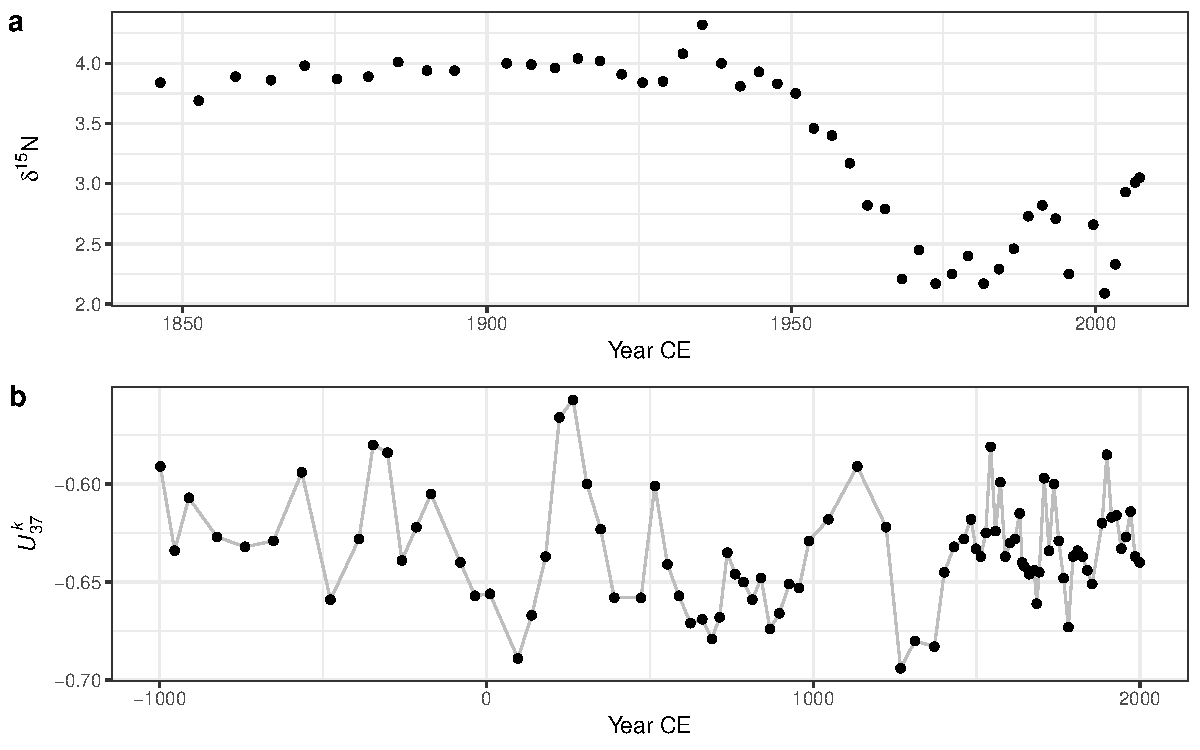
\includegraphics[width=0.8\linewidth]{manuscript_files/figure-latex/data-figure-1} 

}

\caption{Example time series; a) Small Water bulk organic matter $\delta^{15}\text{N}$ time series on a ${}^{210}\text{Pb}$ time scale, and b) Braya-Sø \uk{} time series on a calibrated ${}^{14}\text{C}$ time scale. The observations \uk{} time series have been joined by lines purely as a visual aid to highlight potential trends.}\label{fig:data-figure}
\end{figure}

\section{Regression models for palaeoenvironmental time
series}\label{regression-models-for-palaeoenvironmental-time-series}

A linear model for a trend in a series of \(T\) observations \(y_t\) at
observation times \(x_t\) with \(t = 1, 2, \ldots, T\) is

\begin{equation} \label{eq:linear-model}
y_t = \beta_0 + \beta_1 x_t + \varepsilon_t \,,
\end{equation}

where \(\beta_0\) is a constant term, the model \emph{intercept},
representing the expected value of \(y_t\) where \(x_t\) is 0.
\(\beta_1\) is the \emph{slope} of the best fit line through the data;
it measures the rate of change in \(y\) for a unit increase in \(x\).
The unknowns, the \(\beta_j\) are commonly estimated using least squares
by minimising the sum of squared errors, \(\sum_t \varepsilon_t^2\). If
we want to ask if the estimated trend \(\beta_1\) is statistically
significant, a process called \emph{inference}, we must make further
assumptions about the data (conditional upon the fitted model) or the
model errors (residuals);
\(\varepsilon_t \stackrel{iid}{\sim} \mathcal{N}(0, \sigma^2)\). This
notation indicates that the residuals \(\varepsilon_t\) are
\emph{independent} and \emph{identically distributed} Gaussian random
variables with mean equal to \(0\) and constant variance \(\sigma^2\).
In the time series setting, the assumption of independence of model
residuals is often violated.

The linear model described above is quite restrictive in terms of the
types of trend it can fit; essentially linear increasing or decreasing
trends, or, trivially, a null trend of no change. This model can be
extended to allow for non-linear trends, most notably by making \(y_t\)
depend on polynomials of \(x_t\), for example

\begin{align} \label{eq:polynomial-model}
y_t &= \beta_0 + \beta_1 x_t + \beta_2 x_t^2 + \cdots + \beta_P x_t^P + \varepsilon_t \\
    &= \beta_0 + \sum_{p = 1}^P \beta_p x_t^p  + \varepsilon_t \,, \nonumber
\end{align}

where polynomials of \(x_t\) up to order \(P\) are used. This model
allows for more complex trends but it remains a fully parametric model
and suffers from several problems, especially the behaviour of the
fitted polynomial at the start and end of the observed series.

Linear models using a range of polynomials fitted to the Small Water
data set are shown in Figure \ref{fig:polynomial-example-plot}. The
low-order models (\(P \in \{1, 3\}\)) result in very poor fit to the
data. The model with \(P = 5\) does a reasonable job of capturing the
gross pattern in the time series, but fails to adapt quickly enough to
the decrease in δ\textsuperscript{15}N that begins \textasciitilde{}1940
CE, and the estimated trend is quite biased as a result. The
\(P = 10\)th-order polynomial model is well able to capture this period
of rapid change, but it does so at the expense of increased complexity
in the estimated trend prior to \textasciitilde{}1940. Additionally,
this model (\(P = 10\)) has undesirable behaviour at the ends of the
series, significantly overfitting the data, a commonly observed problem
in polynomial models such as these (Epperson, 1987; Runge, 1901).
Finally, the choice of what order of polynomial to fit is an additional
choice left for the analyst to specify; choosing the optimal \(P\) is
not a trivial task when the data are a time series and residual
autocorrelation is likely present.

\begin{figure}

{\centering 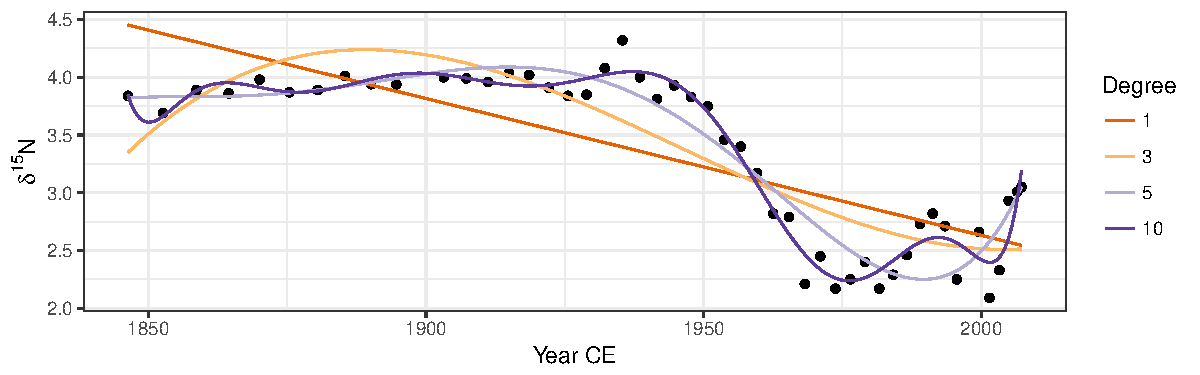
\includegraphics[width=0.8\linewidth]{manuscript_files/figure-latex/polynomial-example-plot-1} 

}

\caption{Linear models with various orders of polynomial of the covariate Year fitted using ordinary least squares to the $\delta^{15}\text{N}$ time series from Small Water. The degree of polynomial is indicated, with the degree 1 line equal to a simple linear regression model.}\label{fig:polynomial-example-plot}
\end{figure}

Can we do better than these polynomial fits? In the remainder, I hope to
demonstrate that the answer to that question is emphatically ``yes''!
Below I describe a coherent and consistent approach to modelling
palaeoenvironmental time series using generalized additive models, which
builds upon the linear regression framework.

\section{Generalized additive models}\label{generalized-additive-models}

The GAM version of the linear model \eqref{eq:linear-model} is

\begin{equation} \label{eq:additive-model}
y_t = \beta_0 + f(x_t) + \varepsilon_t \, ,
\end{equation}

where the linear effect of time(the \(\beta_1 x_t\) part) has been
replaced by a smooth function of time, \(f(x_t)\). The immediate
advantage of the GAM is that we are no longer restricted to the shapes
of trends that can be fitted via global polynomial functions such as
\eqref{eq:polynomial-model}. Instead, the shape of the fitted trend will
be estimated from the data itself.

The linear model is a special case of a broader class know as the
generalized linear model (GLM; McCullagh and Nelder, 1989). The GLM
provides a common framework for modelling a wide range of types of data,
such as count, proportions, or binary (presence/absence) data, that are
not conditionally distributed Gaussian. GLMs are, like the linear model,
parametric in nature; the types of trends that we can fit using a GLM
are the linear or polynomial models. GAMs extend the GLM by relaxing
this parametric assumption; in a GAM some, or all, of the parametric
terms, the \(\beta_p\), are replace by smooth functions \(f_j\) of the
covariates \(x_j\). For completeness then, we can write
\eqref{eq:additive-model} as a GLM/GAM

\begin{subequations}
\label{eq:gam}
\begin{align}
y_t &\sim \text{EF}(\mu_t, \Theta) \label{eq:gam-ef} \\
g(\mu_t) &= \beta_0 + f(x_t) \label{eq:gam-linear-pred} \\
\mu_t    &= g^{-1}(\beta_0 + f(x_t)), \label{eq:gam-inverse} 
\end{align}
\end{subequations}

where \(\mu_t\) is the expected value (e.g.~the mean count or the
probability of occurrence) of the random variable \(Y_t\)
(\(\mu_t \equiv \mathbb{E}(Y_t)\)) of which we have observations
\(y_t\). \(g\) is the link function, an invertible, monotonic function,
such as the natural logarithm, and \(g^{-1}\) is its inverse. The link
function maps values from the response scale on to the scale of the
linear predictor, whilst the inverse of thew link function provides the
reverse mapping. For example, count data are strictly non-negative
integer values and are commonly modelled as a Poisson GLM/GAM using the
natural log link function. On the log scale, the response can take any
real value between \(-\infty\) and \(+\infty\), and it is on this scale
that model fitting actually occurs (i.e.~using equation
\eqref{eq:gam-linear-pred}). However we need to map these unbounded
values back on to the non-negative response scale. The inverse of the
log link function, the exponential function, achieves this and maps
values to the interval 0--\(\infty\) (equation \eqref{eq:gam-inverse}).

In \eqref{eq:gam-ef}, we further assume that the observations are drawn
from a member of the exponential family of distributions --- such as the
Poisson for count data, the binomial for presence/absence or counts from
a total --- with expected value \(\mu_t\) and possibly some additional
parameters \(\Theta\) (\(y_t \sim \text{EF}(\mu_t, \Theta)\)).
Additionally, many software implementations of the above model also
allow for distributions that are not within the exponential family but
which can be fitted using an algorithm superficially similar to the one
used to fit GAMs to members of the exponential family (e.g. Wood et al.,
2016). Common examples of such extended families include the negative
binomial distribution (for overdispersed counts) and the beta
distribution (for true proportions or other interval-bounded data).

\subsection{Basis functions}\label{basis-functions}

It is clear from the plots of the data that we require the fitted trends
for the Small Water δ\textsuperscript{15}N and Braya-Sø \uk{} time
series to be non-linear functions, but it is less clear how to specify
the actual shape require. Ideally, we'd like to learn the shape of the
trend from the data themselves. We will refer to these non-linear
functions as \emph{smooth functions}, or just \emph{smooths} for short,
and we will denote a smooth using \(f(x_t)\). Further, we would like to
represent the smooths in a way that \eqref{eq:gam} is represented
parametrically so that it can be estimate within the well-studied GLM
framework. This is achieved by representing the smooth using a
\emph{basis}. A basis is a set of functions that collectively span a
space of smooths that, we hope, contains the true \(f(x_t)\) or a close
approximation to it. The functions in the basis are known as \emph{basis
functions}, and arise from a \emph{basis expansion} of a covariate.
Writing \(b_j(x_t)\) as the \(j\)th basis function of \(x_t\), the
smooth \(f(x_t)\) can be represented as a weighted sum of basis
functions

\begin{equation*}
f(x_t) = \sum_{j = 1}^{k} b_j(x_t) \beta_j \,,
\end{equation*}

where \(\beta_j\) is the weight applied to the \(j\)th basis function.
Note that here we concern ourselves only with univariate smooths
involving a single covariate, the time variable \(x_t\).

The polynomial model we encountered earlier is an example of a
statistical model that uses a basis expansion. For the cubic polynomial
(\(P = 3\)) fit shown in Figure \ref{fig:polynomial-example-plot} there
are in fact 4 basis functions: \(b_1(x_t) = x_t^0 = 1\),
\(b_2(x_t) = x_t\), \(b_3(x_t) = x^2_t\), and \(b_4(x_t) = x_t^3\). Note
that \(b_1(x_t)\) is constant and is linked to the model intercept,
\(\beta_0\), in the linear model \eqref{eq:polynomial-model}, and
further, that the weights are the estimated coefficients in the model,
the \(\beta_j\).

As we have already seen, polynomial basis expansions do not necessarily
lead to well-fitting models unless the true function \(f\) is itself a
polynomial. One of the primary criticisms is that polynomial basis
functions are global (Magee, 1998); the value of \(f\) at time point
\(x_t\) affects the value of \(f\) at time point \(x_{t+s}\) even if the
two time points are at opposite ends of the series. There are many other
bases we could use; here I discuss one such set of bases, that of
splines.

There are a bewildering array of different types of spline. In the
models discussed below we will largely restrict ourselves to cubic
regression splines (CRS) and thin plate regression splines (TPRS). In
addition, I also discuss two special types of spline basis, an adaptive
spline basis and a Gaussian process spline basis.

A cubic spline is a smooth curve comprised of sections of cubic
polynomials (\(P = 3\)), where the sections are joined together at some
specified locations --- known as \emph{knots} --- in such a way that at
the joins, the two sections of cubic polynomial that meet have the same
value as well as the same first and second derivative. These properties
mean that the sections join smoothly and differentiably at the knots
(Wood, 2017, 5.3.1).

\begin{figure}

{\centering 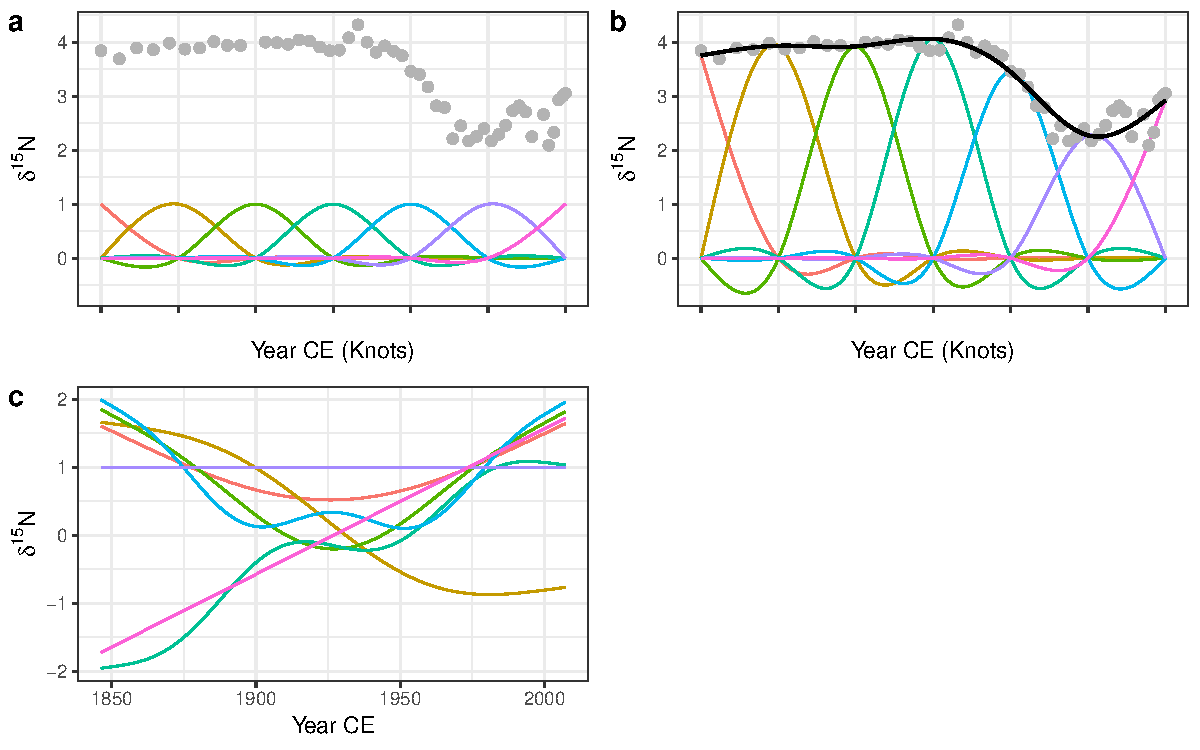
\includegraphics[width=0.8\linewidth]{manuscript_files/figure-latex/basis-function-example-plot-1} 

}

\caption{Basis functions for the time covariate and the Small Water $\delta^{15}\text{N}$ time series. A rank (size) 7 cubic regression spline (CRS) basis expansion is show in a), with knots, indicated by tick marks on the x-axis, spread evenly through the rang of the data. b) shows the same CRS basis functions weighted by the estimated coefficients $\beta_j$, plus the resulting GAM trend line (black line drawn through the data). The grey points in both panels are the observed $\delta^{15}\text{N}$ values. c) A rank 7 thin plate regression spline basis for the same data.}\label{fig:basis-function-example-plot}
\end{figure}

The CRS can be parameterized in a number of different ways. One requires
a knot at each unique data value in \(x_t\), which is computationally
inefficient. Another way of specifying a CRS basis is to parameterize in
terms of the value of the spline at the knots. Typically in this
parametrization there are many fewer knots than unique data, with the
knots distributed evenly over the range of \(x_t\) or at the quantiles
of \(x_t\). Placing knots at the quantiles of \(x_t\) has the effect of
placing a greater number of knots where the data is densest.

A CRS basis expansion comprised of 7 basis functions for the time
covariate in the Small Water series, is shown in Figure
\ref{fig:basis-function-example-plot}a. The tick marks on the x-axis
show the locations of the knots, which are located at the ends of the
series and evenly in between. Notice that in this particular
parametrization, the \(j\)th basis function takes a value of 1 at the
\(j\)th knot and at all other knots a value of 0.

To estimate a model using this basis expansion each basis function forms
a column in the model matrix \(\boldsymbol{X}\) and the weights
\(\beta_j\) can be found using least squares regression (assuming a
Gaussian response). Note that in order to estimate a coefficient for
each basis function the model has to be fitted without an intercept
term. In practice we would include an intercept term in the model and
therefore the basis functions are modified via an identifiability
constraint. This has the effect of making the basis orthogonal to the
intercept but results in more complicated basis functions than those
shown in in Figure \ref{fig:basis-function-example-plot}a.

Having estimated the weight for each basis function, the \(j\)th basis
function \(b_j\) is scaled (weighted) by its coefficient \(\beta_j\).
The scaled CRS basis functions for the Small Water time series are shown
in Figure \ref{fig:basis-function-example-plot}b. The solid line passing
through the data points is formed by summing up the values of the scaled
basis functions (\(b_j(x_t) \beta_j\)) at any value of \(x_t\) (time).

Cubic regression splines, as well as many other types of spline, require
the analyst to choose the number and location of the knots that
parametrise the basis. Thin plate regression splines (TPRS) remove this
element of subjectivity when fitting GAMs. Thin plate splines were
introduced by Duchon (1977) and, as well as solving the knot selection
problem, have several additional attractive properties in terms of
optimality and their ability to estimate a smooth function of two or
more variables, leading to smooth interactions between covariates.
However, thin plate splines have one key disadvantage over CRS; thin
plate splines have as many unknown parameters as there are unique
combinations of covariate values in a data set (Wood, 2017, 5.5.1). It
is unlikely in the extreme that any real data problem would involve
functions of such complexity that they require as many basis functions
as data. It is much more likely that the true functions that we attempt
to estimate are far simpler than the set of functions representable by 1
basis function per unique data value. From a practical point of view, it
is also highly inefficient to carry around all these basis functions
whilst model fitting, and the available computational resources would
become quickly exhausted for large time series with many observations.

To address this issue, thin plate regression splines (TPRS) have been
suggested which truncate the space of the thin plate spline basis to
some lower number of basis functions whilst preserving much of the
advantage of the original basis as an optimally-fitting spline (Wood,
2003). A rank 7 TPRS basis (i.e.~one containing 7 basis functions) is
shown in Figure \ref{fig:basis-function-example-plot}c for the Small
Water time series. The truncation is achieved by performing an
eigen-decomposition of the basis functions and retaining the
eigenvectors associated with the \(k\) largest eigenvalues. This is
similar to the way principal components analysis decomposes a data set
into axes of variation (eigenvectors) in decreasing order of variance
explained. The truncated basis can preserve much of the space of
functions spanned by the original basis but at the cost of using far
fewer basis functions (Wood, 2003, 2017, 5.5.1). Note the horizontal
TPRS basis function (at δ\textsuperscript{15}N = 1) in Figure
\ref{fig:basis-function-example-plot}c; this basis function is
confounded with the intercept term and, after the application of
identifiability constraints, ends up being removed from the set of basis
functions used to fit the model.

The truncation suggested by Wood (2003) is not without cost; the
eigen-decomposition and related steps can be relatively costly for large
data sets. For data sets of similar size to the two examples used here,
the additional computational effort required to set up the TPRS basis
over the CRS basis will not be noticeable. For highly resolved series
containing more than \textasciitilde{}1000 observations the truncation
may be too costly computationally. In such instances, little is lost by
moving to the CRS basis, with the same number of knots as the rank of
the desired TPRS, with the benefit of considerably reduced set up time
for the basis.

To fit a GAM using either of the two regression spline bases described
above, the analyst is generally only required to the specify the size
(rank) of the basis expansion required to represent or closely
approximate the true function \(f\). With practice and some knowledge of
the system from which the observations arise, it can be relatively easy
to put an upper limit on the expected complexity of the true trend in
the data. Additionally, the number available data points places a
constraint on the upper limit of the size of basis expansion that can be
used.

In practice, the size of the basis is an upper limit on the expected
complexity of the trend, and a simple test is available to check if the
basis used was sufficiently large (Pya and Wood, 2016). This test is
available via the \texttt{gam.check()} function in \emph{mgcv} for
example, which essentially looks at whether there is any additional
nonlinearity or structure in the residuals that can be explained by a
further smooth of \(x_t\). Should a smooth term in the fitted model fail
this test the model can be refitted using a larger basis expansion, say
by doubling the value of \emph{k} (the rank) used to fit the original.
Note also that a smooth might fail this test whilst using fewer
effective degrees of freedom than the maximum possible for the dimension
of basis used. This may happen when the true function lies at the upper
limit of the set of functions encompassed by the size of basis used.
Additionally, a basis of size \(2k\) encompasses a richer space of
functions of a given complexity than a basis of size \(k\) (Wood, 2017);
increasing the basis dimension used to fit the model may unlock this
additional function space resulting in a better fitting model whilst
using a similar number of effective degrees of freedom.

\subsection{Smoothness selection}\label{smoothness-selection}

Having identified regression splines as a useful way to represent \(f\),
we next need a way to decide how wiggly the fitted trend should be. A
backwards elimination approach to sequentially remove knots or basis
functions might seem appropriate, however such an approach would likely
fail as the resulting sequence of models would not be strictly nested,
precluding many forms of statistical comparison (Wood, 2017).
Alternatively, we could keep the basis dimension at a fixed size but
guard against fitting very complex models through the use of a
wiggliness penalty.

The default wiggliness penalty used in GAMs is on the second derivative
of the spline, which measures the rate of change of the slope, or the
curvature, of the spline at any infinitesimal point in the interval
spanned by \(x_t\). The actual penalty used is the integrated squared
second derivative of the spline

\begin{equation} \label{eq:quadratic-penalty}
\int_{\mathbb{R}} [f^{\prime\prime}]^2 dx = \boldsymbol{\beta}^{\mathsf{T}}\mathbf{S}\boldsymbol{\beta}\, .
\end{equation}

The right hand side of \eqref{eq:quadratic-penalty} is the penalty in
quadratic form. The convenience of the quadratic form is that it is a
function of the estimated coefficients of \(f(x_t)\) where
\(\mathbf{S}\) is known as the penalty matrix. Notice that now both the
weights for the basis functions and the wiggliness penalty are expressed
as functions of the model coefficients.

Now that we have a convenient way to measure wiggliness, it needs to be
incorporated into the objective function that will be minimised to fit
the GAM. The likelihood of the model given the parameter estimates
\(\mathcal{L}(\boldsymbol{\beta})\) is combined with the penalty to
create the penalized likelihood \(\mathcal{L}_p(\boldsymbol{\beta})\):

\begin{equation*}
\mathcal{L}_p(\boldsymbol{\beta}) = \mathcal{L}(\boldsymbol{\beta}) - \frac{1}{2} \lambda\boldsymbol{\beta}^{\mathsf{T}}\mathbf{S}\boldsymbol{\beta}\, .
\end{equation*}

The fraction of a half is there simply to make the penalised likelihood
equal the penalised sum of squares in the case of a Gaussian model.
\(\lambda\) is known as the smoothness parameter and controls the extent
to which the penalty contributes to the likelihood of the model. In the
extreme case of \(\lambda = 0\) the penalty has no effect and the
penalized likelihood equals the likelihood of the model given the
parameters. At the other extreme, as \(\lambda \rightarrow \infty\) the
penalty comes to dominate \(\mathcal{L}_p(\boldsymbol{\beta})\) and the
wiggliness of \(f(x_t)\) tends to \(0\) resulting in an infinitely
smooth function. In the case of a second derivative penalty, this is a
straight line, and we recover the simple linear trend from
\eqref{eq:linear-model} when assuming a Gaussian response.

\begin{figure}

{\centering 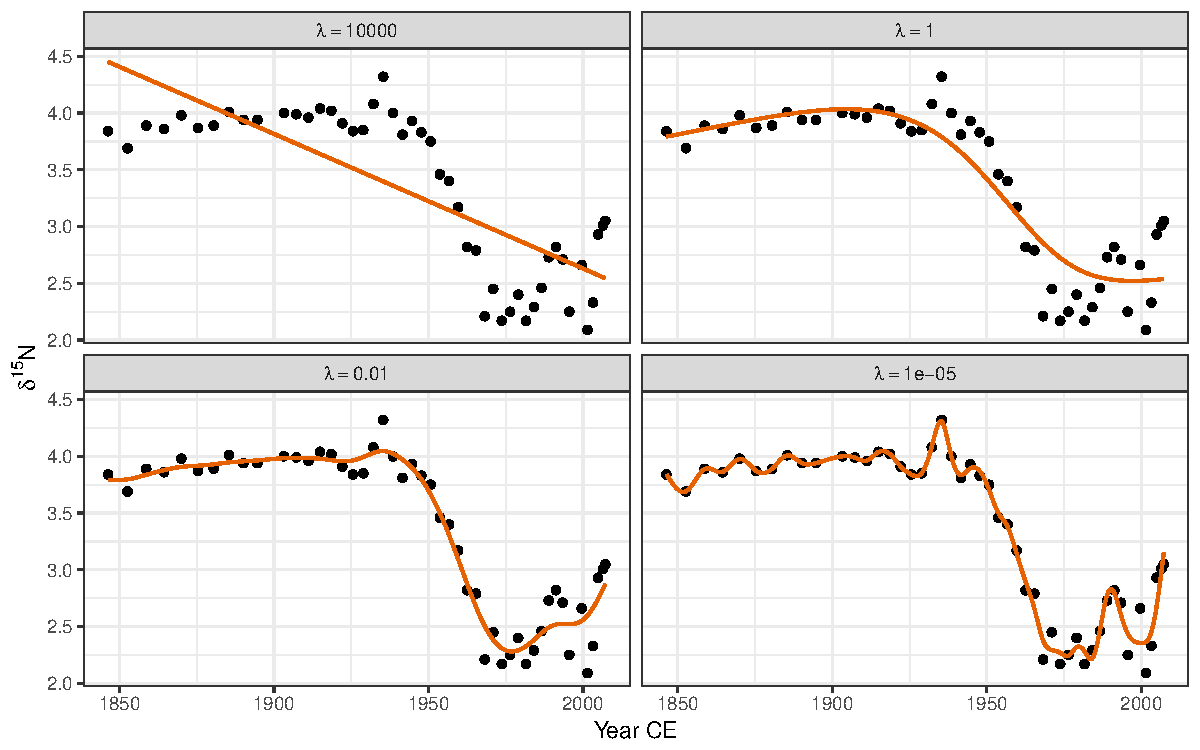
\includegraphics[width=0.8\linewidth]{manuscript_files/figure-latex/penalty-example-plot-1} 

}

\caption{The effect of the smoothness parameter $\lambda$ on the resulting wiggliness of the estimated spline. Large values of $\lambda$ penalize wiggliness strongly, resulting in smooth trends (upper row), while smaller values allow increasingly wiggly trends. The aim of automatic smoothness selection is to find an optimal value of $\lambda$ that balances the fit of the model with model complexity to avoid overfitting.}\label{fig:penalty-example-plot}
\end{figure}

Figure \ref{fig:penalty-example-plot} illustrates how the smoothness
parameter \(\lambda\) controls the degree of wiggliness in the fitted
spline. Four models are shown, each fitted with a fixed value of
\(\lambda\); 10000, 1, 0.01, and 0.00001. At \(\lambda = 10000\) the
model effectively fits a linear model through the data. As the value of
\(\lambda\) decreases, the fitted spline becomes increasingly wiggly. As
\(\lambda\) becomes very small, the resulting spline passes through most
of the δ\textsuperscript{15}N observations resulting in a model that is
clearly over fitted to the data.

To fully automate smoothness selection for \(f(x_t)\) we need to
estimate \(\lambda\). There are two main ways that \(\lambda\) can be
automatically chosen during model fitting. The first way is to choose
\(\lambda\) such that it minimises the prediction error of the model.
This can be achieved by choosing \(\lambda\) to minimise Akaike's
information criterion (AIC) or via cross-validation (CV) or generalized
cross-validation (GCV; Craven and Wahba, 1978). GCV avoids the
computational overhead inherent to CV of having to repeatedly refit the
model with one or more observations left out as a test set. Minimising
the GCV score will, with a sufficiently large data set, find a model
with the minimal prediction error (Wood, 2017). The second approach is
to treat the smooth as a random effect, in which \(\lambda\) is now a
variance parameter to be estimated using maximum likelihood (ML) or
restricted maximum likelihood (REML; Wood, 2011; Wood et al., 2016).

Several recent results have shown that GCV, under certain circumstances,
has a tendency to under smooth, resulting in fitted splines that are
overly wiggly (Reiss and Ogden, 2009). Much better behaviour has been
observed for REML and ML smoothness selection, in that order (Wood,
2011). REML is therefore the recommended means of fitting GAMs, though,
where models have different fixed effects (covariates) they cannot be
compared using REML, and ML selection should be used instead. In the
sorts of data examples considered here there is only a single covariate
\(x_t\) as our models contain a single estimated trend so REML
smoothness selection is used throughout unless otherwise stated.

\section{Fitting GAMs}\label{fitting-gams}

\subsection{Small Water}\label{small-water}

The trend in δ\textsuperscript{15}N values is clearly non-linear and it
would be difficult to suggest a suitable polynomial model that would
allow for periods of relatively no change in δ\textsuperscript{15}N as
well as rapid change. Instead, a GAM is ideally suited to modelling such
trends; the data suggest a smoothly varying change in
δ\textsuperscript{15}N between 1925 and 1975. It is reasonable to expect
some autocorrelation in the model errors about the fitted trend.
Therefore I fitted the following GAM to the δ\textsuperscript{15}N time
series.

\begin{equation} \label{eq:small-gam}
y_t = \beta_0 + f(x_t) + \varepsilon, \quad \varepsilon_t \sim \mathcal(0, \boldsymbol{\Lambda}\sigma^2)
\end{equation}

Note that now I have relaxed the i.i.d. assumption and have introduced
\(\boldsymbol{\Lambda}\), a correlation matrix that is used to model
autocorrelation in the residuals. The δ\textsuperscript{15}N values are
irregularly spaced in time and a correlation structure that can handle
the uneven spacing of the samples is needed (Pinheiro and Bates, 2000).
A continuous time first-order autoregressive process (CAR(1)) is a
reasonable choice; it is the continuous-time equivalent of the
first-order autoregressive process (AR(1)) and, simply stated, models
the correlation between any two residuals as and exponentially
decreasing function of \(h\) (\(\phi^h\)), where \(h\) is the amount of
separation in time between the residuals (Pinheiro and Bates, 2000).
\(h\) may be a real valued number in the CAR(1), which is how it can
accommodate the irregular separation of samples in time. \(\phi\)
controls how quickly the correlation between any two residuals declines
as a function of their separation in time and is an additional parameter
that will be estimated during model fitting. The model in
\eqref{eq:small-gam} was fitted using the \texttt{gamm()} function
(Wood, 2004) in the \emph{mgcv} package (Wood, 2017) for R (R Core Team,
2017).

\begin{figure}

{\centering 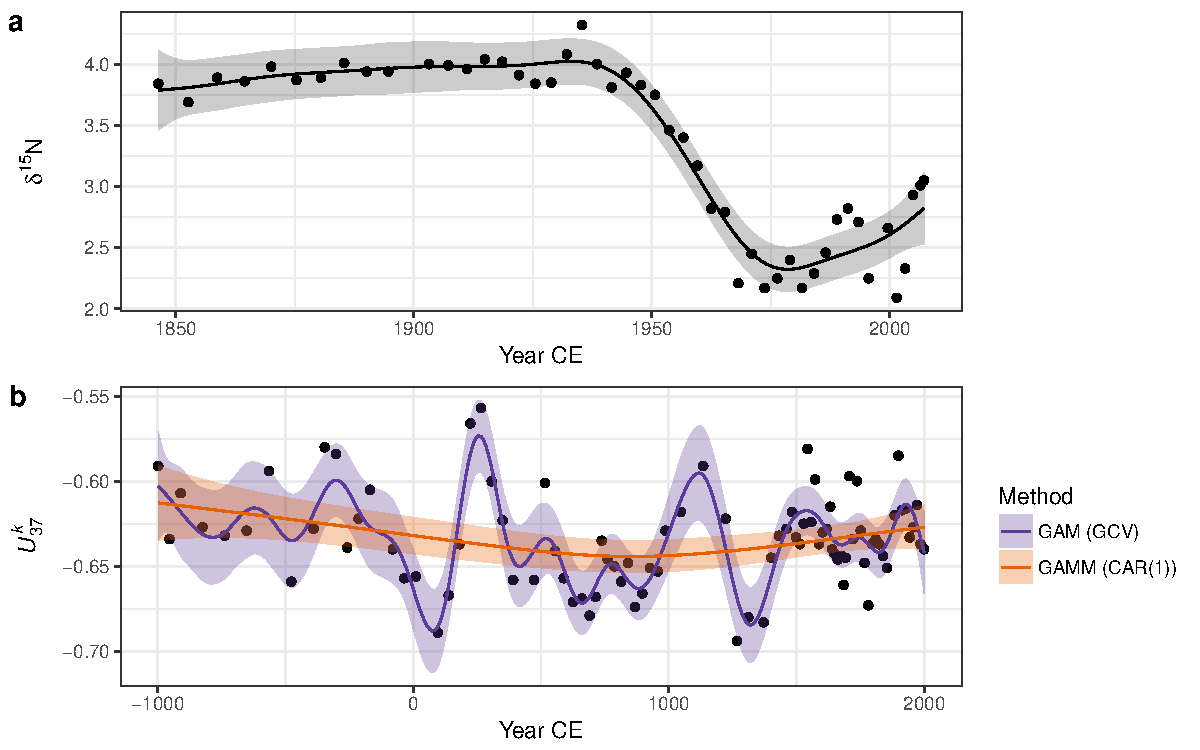
\includegraphics[width=0.8\linewidth]{manuscript_files/figure-latex/plot-fitted-models-1} 

}

\caption{GAM-based trends fitted to the Small Water $\delta^{15}\text{N}$ (a) and Braya-Sø \uk{} (b) time series. The shaded bands surrounding the estimated trends are approximate 95\% across-the-function confidence intervals. For the \uk{} series, two models are shown; the orange fit is the result of a GAM with a continuous-time AR(1) process estimated using REML smoothness selection, while the blue fit is that of a simple GAM with GCV-based smoothness selection. The REML-based fit significantly oversmooths the \uk{} time series.}\label{fig:plot-fitted-models}
\end{figure}

The fitted trend is shown in Figure \ref{fig:plot-fitted-models}a, and
well-captures the strong pattern in the data. The trend is statistically
significant (estimated degrees of freedom = 7.95; \(F\) = 47.44,
approximate \(p\) value = \(\ll\) 0.0001). However further analysis of
the fitted model is required to answer the other questions posed earlier
about the timing of change and whether features in the trend can be
distinguished from random noise. I discuss these issues shortly.

\subsection{Braya-Sø}\label{braya-s}

The \uk{} data present a more difficult data analysis challenge than the
δ\textsuperscript{15}N time series because of the much more complex
variation present. Fitting the same model as the Small Water example,
\eqref{eq:small-gam}, to the \uk{} data resulted in the unsatisfactory
fit shown as the very smooth line in Figure
\ref{fig:plot-fitted-models}b (labelled GAMM (CAR(1))). Further problems
were evident with this model fit --- the covariance matrix of the model
was non-positive definite, a sure sign of problems with the fitted
model. Refitting with a smaller basis dimension (\emph{k} = 20) for the
trend term resulted in a model with a positive-definite covariance
matrix for the model variance-covariance terms, but the estimated value
of of the CAR(1) parameter \(\phi\) = 0.2 was exceedingly uncertain
(95\% confidence interval 0 -- 1!)

Fitting this model as a standard GAM with REML smoothness selection
resulted in the same fitted trend as the GAM with CAR(1) errors (not
shown), whilst using GCV smoothness selection resulted in a much more
satisfactory fitted trend. There are two potential problems with the
GCV-selected trend: i) GCV is sensitive to the profile of the GCV score
and has been shown to badly under smooth data in situations where the
profile is flat around the minimum GCV score, and ii) the model fitted
assumes that the observations are independent, an assumption that is
certainly violated in the \uk{} time series.

To investigate the first issue, the GCV and REML scores for an
increasing sequence of values of the smoothness parameter (\(\lambda\))
were evaluated for the standard GAM (equation \eqref{eq:gam}) fit to the
\uk{} time series. The resulting profiles are shown in Figure
\ref{fig:trace-smoothness-parameters}, with the optimal value of the
parameter shown by the vertical line. The GCV score profile suggests
that the potential for under smoothing identified by Reiss and Ogden
(2009) is unlikely to apply here as there is a well-defined minimum in
profile. Addressing the violation of the independence assumption is more
difficult; the standard errors of the model coefficients are most likely
anti-conservative, which presents a significant problem if we wish to
determine which of the wiggles in the fitted \uk{} trend can be
identified as real.

To understand the reason why the GAM plus CAR(1) and the simple GAM with
REML smoothness selection performed poorly with the \uk{} time series we
need to delve a little deeper into what is happening when we are fitting
these two models.

\begin{figure}

{\centering 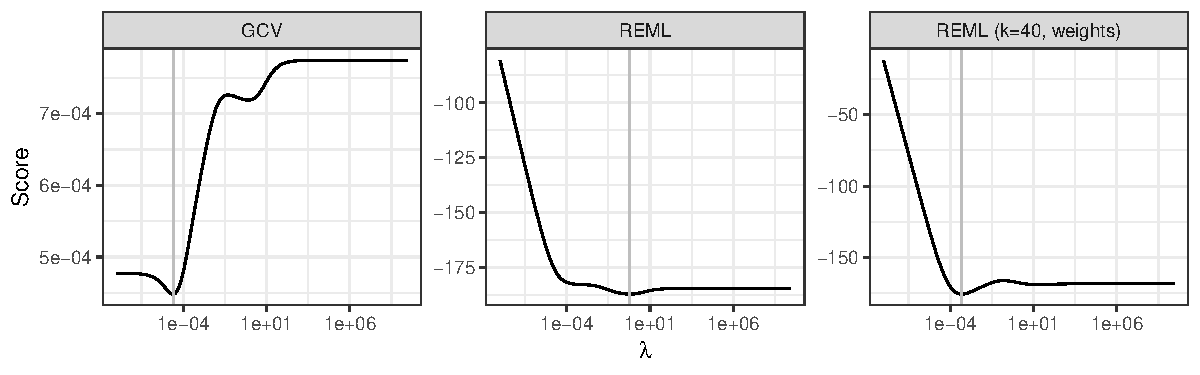
\includegraphics[width=0.8\linewidth]{manuscript_files/figure-latex/trace-smoothness-parameters-1} 

}

\caption{GCV and REML scores as a function of the smoothness parameter $\lambda$. From left to right, GAMs were estimated using GCV and REML smoothness selection, and REML using a basis dimension of 40 and observational weights to account for heterogeneity in the \uk{} times series. The selected value of $\lambda$ for each model is indicated by the vertical grey line.}\label{fig:trace-smoothness-parameters}
\end{figure}

The primary issue leading to poor fit is that neither model accounts for
the different variance (known as (heteroscedasticity) of each
observation in the \uk{} record. The sediments in Braya-Sø are not
annually laminated and therefore the core was sliced at regular depth
intervals. Owing to compaction of older sediments and variation in
accumulation rates over time, each sediment slice represents a different
number of ``lake years''. We can think of older samples as representing
some average of many years of sediment deposition, whilst younger
samples are representative of fewer of these lake years. The average of
a larger set of numbers is estimated more precisely than the average of
a smaller set, all things equal. A direct result of this variable
averaging of lake years it that some samples are more precise and
therefore have lower variance than other samples and yet the model
assumed that the variance was constant across samples.

Accounting for heteroscedasticity within the model is relatively simple
via the use of observational weights. The number of lake years
represented by each slice is estimated by assigning a date to the top
and bottom of each sediment slice. The variance of each observation
should be proportional to the inverse of the number of lake years each
sample represents. In the \texttt{gam()} function used here, weights
should be specified as the number of lake years each sample represents.
Other software may require the weights to be specified in a different
way.

A secondary problem is the size of the basis dimension used for the time
variable. The main user selectable option when fitting a GAM in the
penalised likelihood framework of Wood (2004) is how many basis
functions to use. As described above, the basis should be large enough
to contain the true, but unknown, function, or a close approximation to
it. For GCV selection the basis used contained 29 basis functions,
whilst the CAR(1) model with REML smoothness selection would only
converge with a basis containing 20 functions. The size of the basis
appears to be sufficient for GCV smoothness selection, but following
Wood (2011) REML smoothness selection is preferred. Using the test of
Pya and Wood (2016), the basis dimension for the models with REML
smoothness selection was too small. To proceed therefore, we must drop
the CAR(1) term and increase the basis dimension to 39 functions (by
setting \texttt{k\ =\ 40}; I set it larger than expected wiggliness
because the larger basis contains a richer family of functions and the
excess complexity is reduced because of the smoothness penalty in play.)

With the larger basis dimension and accounting for the non-constant
variance of the observations via weights, the model fitted using REML is
indistinguishable from that obtained using GCV (Figure
\ref{fig:plot-fitted-models}b). The trace of the REML score for this
model (Figure \ref{fig:trace-smoothness-parameters}c) shows a pronounced
minimum at a much smaller value of \(\lambda\) than the original REML
fit (Figure \ref{fig:trace-smoothness-parameters}b), indicating that a
more wiggly trend provides a better fit to the Braya-Sø time series.
This example illustrates that some care and understanding of the
underlying principles of GAMs is required to diagnose potential issues
with the estimated model. After standard modelling choices (size of
basis to use, correct selection of response distribution and link
function, etc.) are checked, it often pays to think carefully about the
properties of the data and ensure that the assumptions of the model are
met. Here, despite increasing the basis size, it was the failure to
appreciate the magnitude of the effect on fitting of the non-constant
variance that lead to the initially poor fit and the problems associated
with the estimation of the CAR(1) process. I return to the issue of why
the GAM plus CAR(1) model encountered problems during fitting later
(\protect\hyperlink{identifiability}{see Identifiability}).

\hypertarget{confints}{\subsection{Confidence intervals and uncertainty
estimation}\label{confints}}

If we want to ask whether either of the estimated trends is
statistically interesting or proceed to identifying periods of
significant change, we must address the issue of uncertainty in the
estimated model. What uncertainty is associated with the trend
estimates? One way to visualise this is through a 1 - \(\alpha\)
confidence interval around the fitted trend, where \(\alpha\) is say
0.05 leading to a 95\% interval. A 95\% interval would be drawn at
\(\hat{y}_t \pm (m_{1-\alpha} \times \text{SE}(\hat{y}_t))\), with
\(m_{1-\alpha} = 1.96\), the 0.95 probability quantile of a standard
normal distribution, and \(\text{SE}(\hat{y}_t)\) is the standard error
of the estimated trend at time \(x_t\). This type of confidence interval
would normally be described as \emph{pointwise}; the coverage properties
of the interval are correct for a single point on the fitted trend, but,
if we were to consider additional points on the trend, the coverage
would logically be lower than 1 - \(\alpha\). This is the traditional
frequentist interpretation of a confidence interval. However, the
approach to fitting GAMs described here has a Bayesian interpretation
(Kimeldorf and Wahba, 1970; Silverman, 1985; Wahba, 1983, 1990) and
therefore the typical frequentist interpretation does not apply. Nychka
(1988) investigated the properties of a confidence interval created as
described above using standard errors derived from the Bayesian
posterior covariance matrix for the estimated mode parameters. Such
intervals have the interesting property that they have good
\emph{across-the-function} coverage when considered from a frequentist
perspective. This means that, when averaged over the range of the
function, the Bayesian credible intervals shown in Figure
\ref{fig:plot-fitted-models} have close to the expected 95\% coverage.
However, to achieve this some parts of the function may have more or
less than 95\%-coverage. Marra and Wood (2012) recently explained
Nychka's (1988) surprising results and extended them to the case of
generalized models (non-Gaussian responses).

\begin{figure}

{\centering 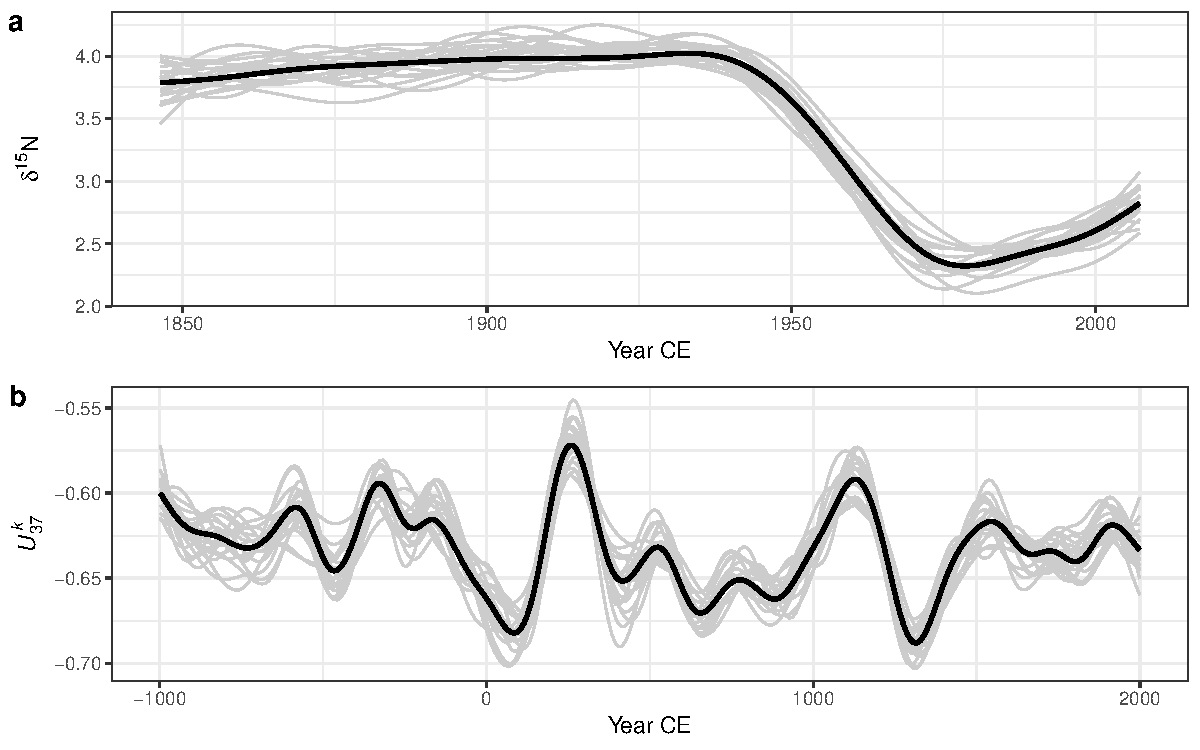
\includegraphics[width=0.8\linewidth]{manuscript_files/figure-latex/posterior-simulation-1} 

}

\caption{Estimated trends (thick black lines) and 20 random draws (grey lines) from the posterior distribution of the GAM fitted to the Small Water $\delta^{15}\text{N}$ (a) and Braya-Sø \uk{} (b) time series.}\label{fig:posterior-simulation}
\end{figure}

Whilst the \emph{across-the-function} or average coverage frequentist
interpretation of the Bayesian credible intervals is useful, if may be
important to have an interval that contains the entirety of the true
function with some state probability (1 - \(\alpha\)). Such an interval
is known as a \emph{simultaneous} interval. A (1 - \(\alpha\))100\%
\emph{simultaneous} confidence interval contains \emph{in their
entirety} 1 - \(\alpha\) of all random draws from the posterior
distribution of the fitted model.

Fitting a GAM involves finding estimates for coefficients of the basis
functions. Together, these coefficients are distributed multivariate
normal with mean vector and covariance matrix specified by the model
estimates of the coefficients and their covariances respectively. Random
draws from this distribution can be taken, where each random draw
represents a new trend that is consistent with the fitted trend but also
includes the uncertainty in the estimated trend. This process is known
as \emph{posterior simulation}.

Figure \ref{fig:posterior-simulation} shows 20 random draws from the
posterior distribution of the GAMs fitted to the Small Water and
Braya-Sø data sets. In the early period of the δ\textsuperscript{15}N
time series many of the posterior simulations exhibit short periods of
increasing and decreasing trend, balancing out to the relatively flat
trend estimated by the GAM (Fig.~\ref{fig:posterior-simulation}a).
Reflecting this uncertainty, we might expect relatively wide
simultaneous intervals during this period in order to contain the vast
majority of the simulated trends. Conversely, the decreasing
δ\textsuperscript{15}N trend starting at \textasciitilde{}1945 is
consistently reproduced in the posterior simulations, suggesting that
this feature of the time series is both real and statistically
significant, and that the rate of change in δ\textsuperscript{15}N is
relatively precisely estimated. We see a similar pattern in
Figure~\ref{fig:posterior-simulation}b for the Braya-Sø record; the
large peak in \uk{} at \textasciitilde{}250CE and the strong decline at
\textasciitilde{}1200CE are well defined in the posterior simulations,
whereas most of the localised trends that are smaller magnitude changes
in \(y_t\) are associated with posterior simulations that are less well
constrained with the ends of the record in particular showing
considerable variation in the strength, timing, and even sign of
simulated trends, reflecting the greater uncertainty in estimated trend
during these periods. For the random draws illustrated in Figure
\ref{fig:posterior-simulation}, a simultaneous interval should contain
the entire function for on average 19 of the 20 draws.

There are a number of ways in which a simultaneous interval can be
computed. Here I follow the simulation approach described by Ruppert et
al. (2003) and present only the basic detail; a fuller description is
contained in Appendix \protect\hyperlink{appendix}{1}. The general idea
is that if we want to create an interval that contains the whole of the
true function with 1 - \(\alpha\) probability, we need to increase the
standard Bayesian credible interval by some amount. We could simulate a
large number of functions from the posterior distribution of the model
and then search for the value of \(m_{1-\alpha}\) that when multiplied
by \(\text{SE}(\hat{f}(x_t))\) yielded an interval that contained the
whole function for \((1-\alpha)\) 100\% of the functions simulated. In
practice, the simulation method of Ruppert et al. (2003) does not
involve a direct search, but yields the critical value \(m_{1-\alpha}\)
required.

\begin{figure}

{\centering 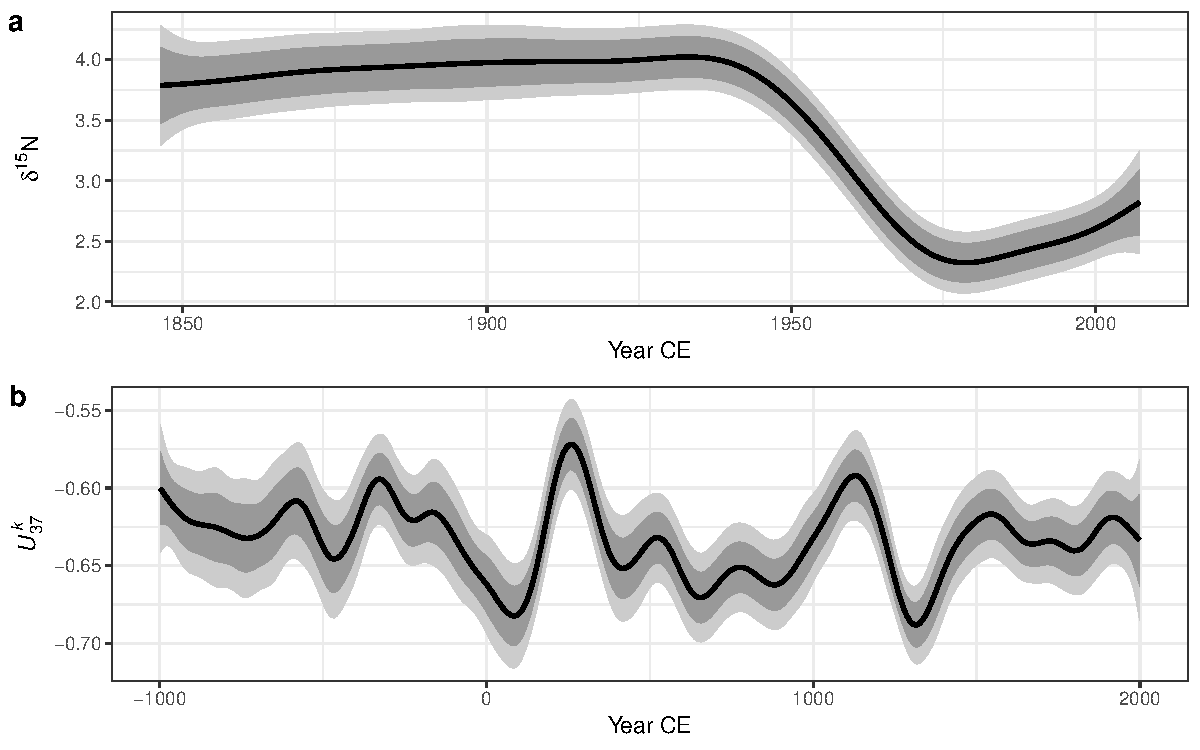
\includegraphics[width=0.8\linewidth]{manuscript_files/figure-latex/compare-intervals-1} 

}

\caption{95\% simultaneous confidence intervals (light grey bands) and across-the-function confidence intervals (dark grey bands) on the estimated trends (black lines) for the Small Water $\delta^{15}\text{N}$ (a) and Braya-Sø \uk{} (b) time series.}\label{fig:compare-intervals}
\end{figure}

Simultaneous intervals computed using the method described are show in
Figure \ref{fig:compare-intervals} alongside the
\emph{across-the-function} confidence intervals for the trends fitted to
both example data sets. As expected, the simultaneous interval is
somewhat wider than the \emph{across-the-function} interval. The
critical value \(m_{1-\alpha}\) for the simultaneous interval of the
estimated trend in δ\textsuperscript{15}N is 3.08, whilst the same value
for the \uk{} series is 3.42, leading to intervals that are
approximately ±50\% and ±75\% wider than the equivalent
across-the-function intervals.

\subsection{Identifying periods
change}\label{identifying-periods-change}

In the simple linear trend model \eqref{eq:linear-model} whether the
estimated trend constitutes evidence for or against a null hypothesis of
no change rests on how large the estimated rate of change in \(y_t\) is
(\(\hat{\beta}_1\)) relative to its uncertainty. This is summarised in
the \(t\) statistic. As the rate of change in \(y_t\) is constant over
the fitted trend --- there is only a singe slope for the fitted trend
\(\hat{\beta}_1\) --- if the \(t\) statistic of the test that
\(\hat{\beta}_1 = 0\) is unusually extreme this would be evidence
against the null hypothesis of no change. Importantly, this applies to
the whole time series as the linear model implies a constant rate of
change throughout. More formally, the estimate \(\hat{\beta}_1\) is the
first derivative of the fitted trend.

In the GAM, the fitted trend need not be linear; the slope of the trend
is potentially different at every point in the time series. As such we
might reasonably ask \emph{where} in the series the response \(y_t\) is
changing, if at all? Mirroring the linear model we can answer this
question by determining whether or not the first derivative at any time
point \(x_t\) of the fitted trend at any time point is consistent with a
null hypothesis of no change. We want to know whether or not the first
derivative is indistinguishable from a value of \(0\) --- no trend ---
given the uncertainty in the estimate of the derivative.

Derivatives of the fitted spline are not easily available analytically,
but they can be estimated using the method of finite differences. Two
values of the estimated trend, separated by a very small time-shift
(\(\Delta_t\)), are predicted from the model; the difference between the
estimated values for the two time points is an approximation of the true
first derivative of the trend. As \(\Delta_t \rightarrow 0\) the
approximation becomes increasingly accurate. In practice, the first
derivative of the fitted trend is evaluated using finite differences at
a large number of points in the time series. An approximate (1 -
\(\alpha\))100\% pointwise confidence interval can be calculated for the
derivative estimates using standard theory
(i.e.~\(\pm 1.96 \times \text{SE}(\hat{y}_t)\) for a 85\% interval) and
the covariance matrix of the spline coefficients. A (1 -
\(\alpha\))100\% simultaneous interval for the derivatives can also be
computed using the method described
\protect\hyperlink{confints}{earlier}. Periods of significant change are
identified as those time points where the (simultaneous) confidence
interval on the first derivative does not include zero.

Figure \ref{fig:derivatives} shows the estimated first derivative of the
fitted trend in the Small Water (\ref{fig:derivatives}a) and Braya-Sø
(\ref{fig:derivatives}b) time series. Although the estimated trend
suggests a slight increase in δ\textsuperscript{15}N from the start of
the record to \textasciitilde{}1940, the estimated trend is sufficiently
uncertain that the simultaneous interval on the first derivative
includes 0 throughout this period. We can understand why this is so by
looking at the posterior simulations in
Figure~\ref{fig:posterior-simulation}a; there is considerable variation
in the shape of the simulated trends throughout this period. From
\textasciitilde{}1925 the derivative of the trend becomes negative,
however it is not until \textasciitilde{}1940 that the simultaneous
interval doesn't include \(0\). At this point we have evidence to reject
the null hypothesis of no change. This time point may be taken as the
first evidence for change in δ\textsuperscript{15}N in the Small Water
core. The simultaneous interval on the first derivative of the trend in
δ\textsuperscript{15}N is bounded away from \(0\) between
\textasciitilde{}1940 and \textasciitilde{}1975, covering the major
decline in values evident in the observations. The simultaneous interval
includes \(0\) from \textasciitilde{}1975 onward, suggesting that,
whilst quite pronounced, the recent increase in δ\textsuperscript{15}N
is not statistically significant. To determine whether or not the recent
increase is real, we would require considerably more samples with which
to (hopefully) more-precisely estimate the trend during this period.
Alternatively, we might just have to wait until sufficient additional
sedimentation has occurred to warrant recoring Small Water and
reestimating the trend in δ\textsuperscript{15}N.

The estimated trend at Braya-Sø exhibited a number of oscillations in
\uk{}. As we saw previously in Figures~\ref{fig:posterior-simulation}b
and \ref{fig:compare-intervals}b, many of these are subject to
significant uncertainty and it is important therefore to discern which,
if any, of the oscillations in the response can be identified given the
model uncertainty. In Figure~\ref{fig:derivatives}b only two features of
the estimated trend are considered significant based on the derivatives
of the smooth; one centred on \textasciitilde{}250CE and a second at
\textasciitilde{}1150CE. In both these periods, the simultaneous
interval for the first derivative of the trend does not include zero. In
the first case we detect the large peak and subsequent decline in \uk{}
at \textasciitilde{}250CE, whilst at \textasciitilde{}1150CE the large
trough is identified, but not the increasing trend immediately prior to
this excursion to lower \uk. Recall that these intervals are
simultaneous in nature, strongly guarding against false positives, and
as such we can be confident in the estimation of these two features,
whilst care must be taken to not over-interpret the remaining variations
in the estimated trend.

\begin{figure}

{\centering 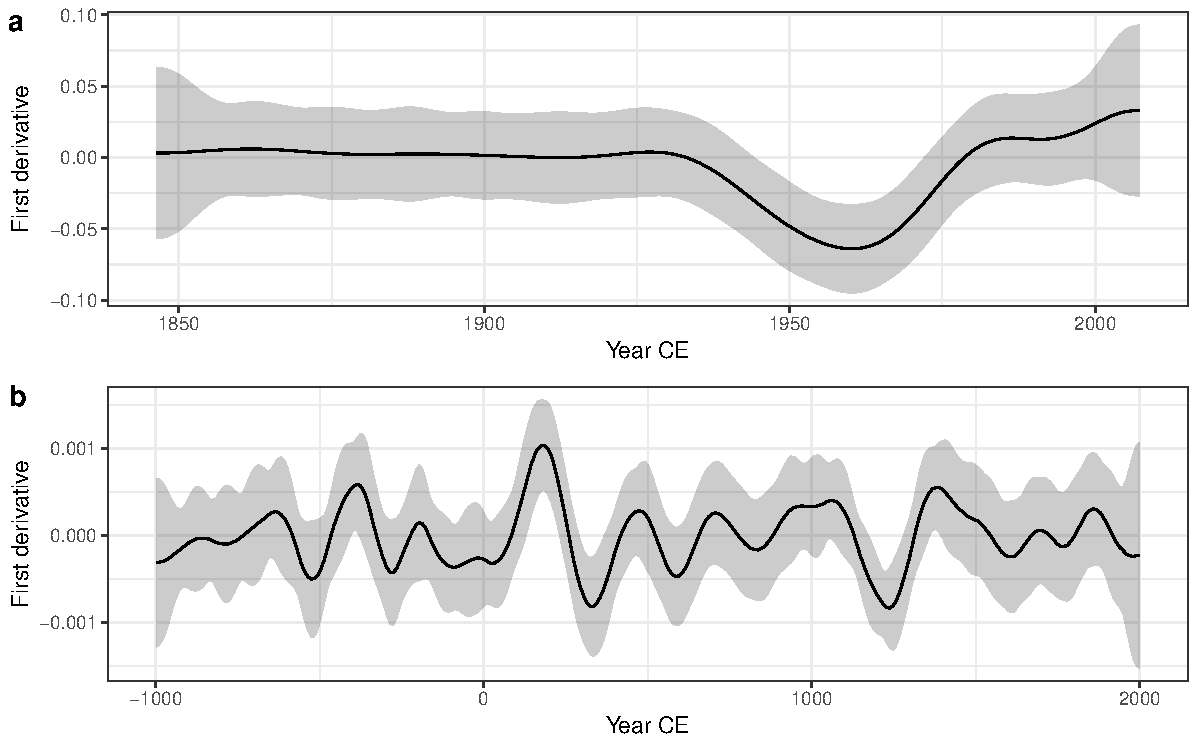
\includegraphics[width=0.8\linewidth]{manuscript_files/figure-latex/derivatives-1} 

}

\caption{Estimated first derivatives (black lines) and 95\% simultaneous confidence intervals of the GAM trends fitted to the Small Water $\delta^{15}\text{N}$ (a) and Braya-Sø \uk{} (b) time series. Where the simultaneous interval does not include 0, the models detect significant temporal change in the response.}\label{fig:derivatives}
\end{figure}

\hypertarget{identifiability}{\subsection{Residual autocorrelation and
model identification}\label{identifiability}}

The GAM fitted to the δ\textsuperscript{15}N time series contained a
CAR(1) process to model residual temporal autocorrelation in the
residuals. The estimated magnitude of the autocorrelation is given by
the parameter \(\phi\). The estimated value of \(\phi\) for the
δ\textsuperscript{15}N series is 0.6 with 95\% confidence interval
0.28--0.85, indicating moderate to strong residual autocorrelation about
the fitted trend. The correlation function is an exponentially
decreasing function of temporal separation (\(\Delta_t\)), and whilst
observations that are a few year apart are quite strongly dependent on
one another, this dependence drops off rapidly as \(\Delta_t\) increases
and is effectively zero when samples are separated by a decade or more
(Figure~\ref{fig:car1-plot}).

Failure to account for the dependencies in the δ\textsuperscript{15}N
time series could lead to the estimation of a more wiggly trend than the
one shown in Figure \ref{fig:plot-fitted-models}a which would negatively
impact the confidence place on the inferences we might draw from the
fitted model. Importantly, failing to account for the strong dependency
in the residuals would lead to smaller uncertainties in the estimated
spline coefficients, which would propagate through to narrower
confidence intervals on the fitted trend and on the first derivatives,
and ultimately to the identification of significant periods of change.
The end result would be a tendency toward anti-conservative
identification of periods of change; the coverage probability would be
lower than the anticipated \(1 - \alpha\), leading to a greater chance
of false positive results.

\begin{figure}

{\centering 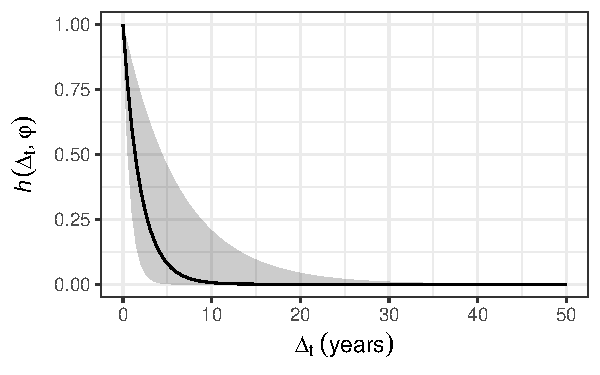
\includegraphics[width=0.5\linewidth]{manuscript_files/figure-latex/car1-plot-1} 

}

\caption{Estimated CAR(1) process from the GAM fitted to the Small Water $\delta^{15}\text{N}$ time series. $h(\Delta_t, \phi)$ is the correlation between residuals separated by $\Delta_t$ years, where $\hat{\phi} = \text{0.6}$. The shaded band is a 95\% pointwise confidence interval on the estimated correlation $h$.}\label{fig:car1-plot}
\end{figure}

Problems estimating the GAM plus CAR(1) model were encountered when this
was fitted to the \uk{} time series; both a smooth trend in the mean
\uk{} and a CAR(1) process in the residuals lead to an unidentifiable
model. What makes a model with a spline-based trend and an
autocorrelation process like the CAR(1) potentially unidentifiable?

Consider again the basic GAM for a smooth trend,
\eqref{eq:additive-model}. In that equation the correlation matrix
\(\boldsymbol{\Lambda}\) was omitted for the sake of simplicity. As I
did in \eqref{eq:small-gam}, I reintroduce it and restate the
distributional assumptions of this model

\begin{equation}
y_t = \beta_0 + f(x_t) + \varepsilon_t, \quad \varepsilon \sim \mathcal(0, \boldsymbol{\Lambda}\sigma^2)
\end{equation}

In the basic GAM, \(\boldsymbol{\Lambda} \equiv \mathbf{I}\) is an
identity matrix, a matrix with 1s on the diagonal and 0s elsewhere

\begin{equation*}
\begin{bmatrix}
1      & 0 & 0 & \dots & 0 \\
0      & 1 & 0 & \dots & 0 \\
0      & 0 & 1 & \dots & 0 \\
\vdots & \vdots & \vdots & \ddots & \vdots \\
0      & 0 & 0 & \dots & 1
\end{bmatrix}\, ,
\end{equation*}

which is where the independence assumption of the model comes from; a
model residual is perfectly correlated with itself (the 1s on the
diagonal), but uncorrelated with any other residual (the off-diagonal
0s). In the GAM plus CAR(1) model, an alternative correlation function
for \(\boldsymbol{\Lambda}\) was used --- the CAR(1) with correlation
parameter \(\phi\). Fahrmeir and Kneib (2008) show that where the
stochastic structure of \(f\) and \(\boldsymbol{\Lambda}\) approach one
another, i.e.~where we have a potentially wiggly trend or strong
autocorrelation as \(\phi \rightarrow 1\), the two processes can quickly
become unidentifiable (see also Fahrmeir et al., 2013). By
unidentifiable, we mean that it becomes increasingly difficult to
distinguish between a wiggly trend or strong autocorrelation because
these two processes are very similar to one another in appearance. This
leads to model estimation problems of the sort encountered with fitting
the GAM plus CAR(1) model to the Braya-sø \uk{} series.

Why might this be so? Autocorrelation is the tendency for a large
(small) value of \(y_t\) at time \(x_t\) to be followed by a likewise
large (small) value at time \(x_{t+1}\). This leads to runs of values
that are consistently greater (less) than the overall mean. Short runs
would indicate weaker autocorrelation whilst longer runs are associated
with stronger autocorrelation, and long runs of values greater (less)
than the mean would evident as non-linear trends in the time series. As
a result, a wiggly trend and an autocorrelation function with large
\(\phi\) are two ways to describe the same pattern of values in a time
series, and without any further information to constrain either the
model is unable to distinguish both components uniquely.

Situations where it may be possible to uniquely identify separate wiggly
trends and autocorrelation are exemplified by the Small Water
δ\textsuperscript{15}N time series. The non-linear trend and the
autocorrelation operate at very different scales; the trend represents
decadal-scale variation in mean δ\textsuperscript{15}N, whilst the
CAR(1) process represents the much smaller-scale tendency for values of
the response to be followed in time by similar values. That such a
pattern is observed in the Small Water core is the result of the high
resolution of the sampling in time relative to the long-term trend. In
contrast, the Braya-Sø record is sampled at far lower resolution
relative to the fluctuations in the mean response, and consequently the
data do not contain sufficient information to separate trend and
autocorrelation.

\subsection{Gaussian process smooths}\label{gaussian-process-smooths}

In the world of machine learning, Gaussian processes (Golding and Purse,
2016; Rasmussen and Williams, 2006) are a widely-used method for fitting
smooth non-parametric regression models. A Gaussian process is a
distribution over all possible smooth functions \(f(x)\). In the field
of spatial statistics, Gaussian processes are known by name
\emph{kriging}.

With a Gaussian process we are interested in fitting a smooth temporal
trend by modelling the way the correlation between pairs of observations
varies as a function of the distance, \(h\), in time that separates
(\(h\)) the observations. The correlation between pairs of observations
decreases with increasing separation, which is modelled using a
correlation function, \(c(h)\). Figure
\ref{fig:gp-correlation-functions} shows examples of two different
correlation functions; the \emph{power exponential} (Figure
\ref{fig:gp-correlation-functions}a), and the Matérn (Figure
\ref{fig:gp-correlation-functions}b) correlation functions. These
functions are smooth and monotonic-decreasing, meaning that the value of
the correlation function decreases with increasing separation (\(h\)).
When \(h\) = 0, the correlation is equal to 1 (\(c(0) = 1\)); two
samples taken at exactly the same time point are perfectly correlated.
As \(h \rightarrow \infty\), the correlation tends to zero
(\(c(h) \rightarrow 0\)); two samples separated by a large amount of
time tend to be uncorrelated. Often we are interested in learning how
large the separation in time needs to be before, on average, a pair of
observations is effectively uncorrelated (i.e.~where \(c(h)\) is
sufficiently close to zero).

\begin{figure}

{\centering 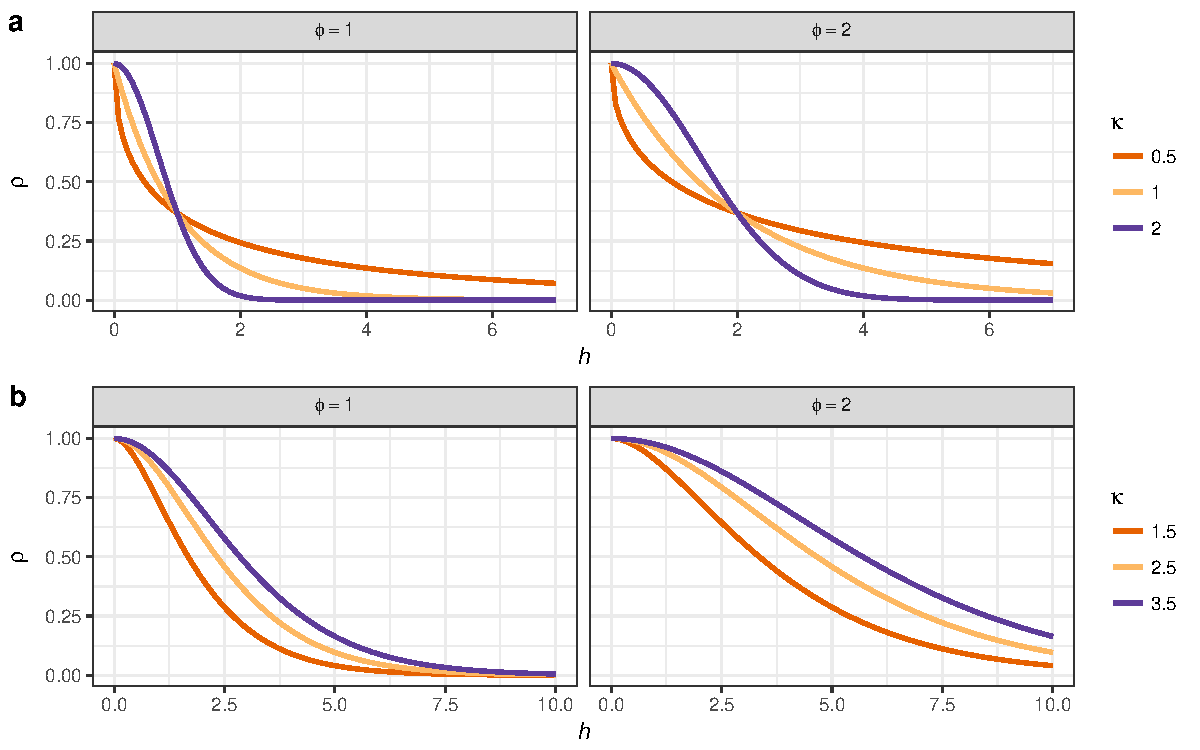
\includegraphics[width=0.8\linewidth]{manuscript_files/figure-latex/gp-correlation-functions-1} 

}

\caption{Power exponential (a) and Matérn (b) correlation functions for observation separation distance $h$. Two values of the effective range parameter ($\phi$)) are shown for each function. For the power exponential function, $\kappa$ is the power in the power exponential function. For the Matérn correlation function, $\kappa$ distinguishes the member of the Matérn family.}\label{fig:gp-correlation-functions}
\end{figure}

Several functions can be used to represent \(c(h)\). Two common ones are
the power exponential function and the Matérn family of correlation
functions. The power exponential function at separation distance \(h\)
is \[c(h) = \exp\{(-h/\phi)^{\kappa}\}\] where \(0 < \kappa \leq 2\).
The Matérn correlation function is actually a family of functions with
closed-forms only available for a subset of the family, distinguished by
\(\kappa\). When \(\kappa = 1.5\), the Matérn correlation function is
\[c(h) = (1 + h/\phi) \exp(-h/\phi)\] whilst for \(\kappa = 2.5\) it is
\[c(h) = \{1 + h/\phi + (h/\phi)^2/3\} \exp(-h/\phi)\] and for
\(\kappa = 3.5\)
\[c(h) = \{1 + h/\phi + 2(h/\phi)^2/5 + (h/\phi)^3/15\} \exp(-h/\phi)\, .\]

In all cases, \(\phi\) is the effective range parameter, which sets the
distance beyond which the correlation function is effectively zero.

\begin{figure}

{\centering 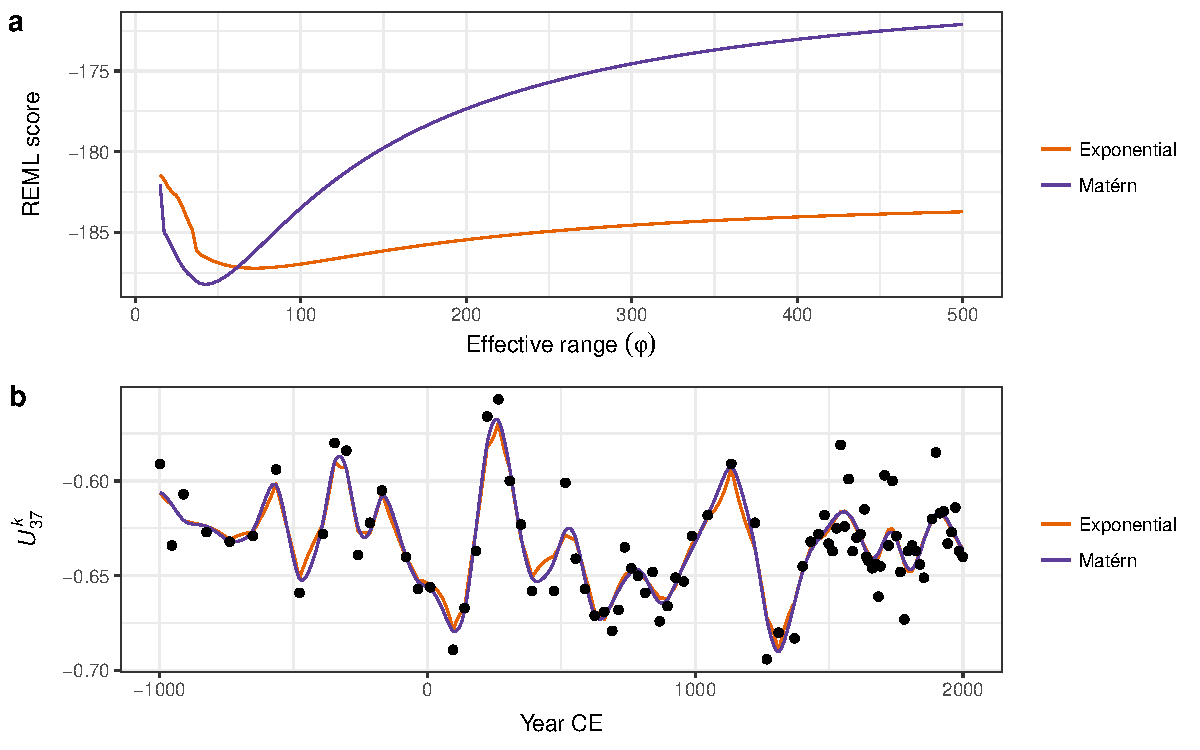
\includegraphics[width=0.8\linewidth]{manuscript_files/figure-latex/gp-gam-detail-plot-1} 

}

\caption{Gaussian process smooths fitted to the \uk{} time series. REML score traces for GAMs fitted using power exponential ($\kappa = 1$) or Matérn ($\kappa = 1.5$) correlation functions as a function of the effective range parameter ($\phi$) are shown (a). The optimal model for each function is that with the lowest REML score. b) shows the resulting trends estimated using the respective correlation function with the value of $\phi$ set to the optimal value.}\label{fig:gp-gam-detail-plot}
\end{figure}

Gaussian processes and GAMs share many similarities and we can fit a
Gaussian process using the techniques already described above for
splines (Handcock et al., 1994; Kammann and Wand, 2003). It can be shown
(e.g. Fahrmeir et al., 2013 section/pages) that the Gaussian process
model has the same penalised likelihood form as the GAM that we
discussed earlier; the observations are the knots of the smoother and
each has a basis function in the form of a correlation function. The
equivalence is only true if the basis functions do not depend on any
other parameters of the model, which is only achievable if the value of
\(\phi\) is fixed and known (Fahrmeir et al., 2013). In general,
however, we would like to estimate \(\phi\) as part of model fitting. To
achieve this we can maximise the profile likelihood or score statistic
of the model over a range of values of \(\phi\) (Wood, 2017, 362--363).
This involves proposing a value of \(\phi\) for the effective range of
the correlation function and then estimating the resulting GAM by
minimising the penalised log-likehood conditional upon this value of
\(\phi\). The model, and its corresponding value of \(\phi\), with
lowest penalised log-likelihood or score statistic is then retained as
the estimated GAM. Figure~\ref{fig:gp-gam-detail-plot}a shows the REML
score for models estimated using a Gaussian process smooth with a Matérn
correlation function (\(\kappa\) = 1.5) for a sequence of values of
\(\phi\) between 15 and 1000 years. There is a clear minimum around 40
years separation, with the minimum REML score being observed at
\(\phi = 41.81)\). Also shown are the REML scores for models using the
power exponential function (\(\kappa\) = 1) with the minimum score
observed at a somewhat higher effective range of \(\phi = 71.06\).

Figure \ref{fig:gp-gam-detail-plot}b shows the estimated trends for the
\uk{} time series using Gaussian process smooths with exponential and
Matérn correlations functions, both using \(\phi\) values at their
respective optimal value as assessed using the REML score. The estimated
trends are very similar to one another, although there is a noticeable
difference in behaviour, with the power exponential (\(\kappa = 1\))
version being noticeably less-smooth than the Matérn version. This
difference is attributable to the shapes of the respective correlation
functions; the Matérn approaches a correlation of 1 smoothly as \(h\)
approaches 0, whilst the power exponential with \(\kappa\) = 1
approaches a correlation of 1 increasingly quickly with decreasing
\(h\). The power exponential with \(\kappa\) = 2, like the Matérn,
approaches \(\phi\) = 1 smoothly, and consequently the trend estimated
using this correlation function is qualitatively similar to that
estimated using the Matérn correlation function.

\subsection{Adaptive smoothing}\label{adaptive-smoothing}

\begin{figure}

{\centering 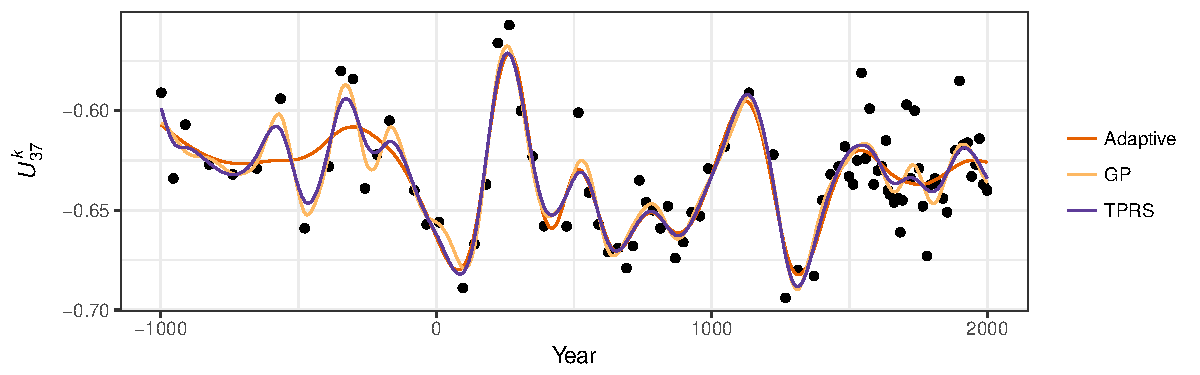
\includegraphics[width=0.8\linewidth]{manuscript_files/figure-latex/braya-so-model-comparisons-1} 

}

\caption{Comparison of trends estimated using i) adaptive smooth, ii) Gaussian process, and iii) thin plate regression spline bases for the \uk{} time series.}\label{fig:braya-so-model-comparisons}
\end{figure}

Each of the spline types that I have discussed so far share a common
feature; the degree of wiggliness over the time series is fixed due to
the use of a single smoothness parameter, \(\lambda\). The definition of
wiggliness, as the integrated squared second derivative of the spline,
ensures that fitted smoother does not jump about wildly. This assumes
that the data themselves are well described by a smoothly varying trend.
If we anticipate abrupt change or step-like responses to environmental
forcing this underlying assumption of the GAM would suggest that the
method is ill-suited to modelling palaeo time series in which such
features are evident or expected.

While there is not much we can do within the GAM framework to model a
series that contains both smooth trends and step-like responses, an
adaptive smoother can help address problems where the time series
consists of periods of rapid change in the mean combined with periods of
complacency or relatively little change. As suggested by their name,
adaptive smoothers can adjust to changes in the wiggliness of the time
series. This adaptive behaviour is achieved by making the smoothness
parameter \(\lambda\) itself depend smoothly on \(x_t\) (Ruppert et al.,
2003, 17; Wood, 2017, 5.3.5); in other words, the adaptive smoother
allows the wiggliness of the estimated trend to vary smoothly over time.
Whilst this does allow the estimated trend to adapt to periods of rapid
change in the response, adaptive smoothers make significant demands on
the data (Wood, 2017, 5.3.5); if we used \(m\) smoothness penalties to
allow the wiggliness to vary over a time series, it would be like
estimating \(m\) separate smooths from chunks of the original series
each of length \(n/m\). In a practical sense, this limits the use of
adaptive splines in palaeoecology to proxies that are readily
enumerated, such as the biogeochemical proxies used in the two example
data sets.

Figure \ref{fig:braya-so-model-comparisons} compares trends for the
Braya-Sø time series estimated using GAMs with the three main types of
spline discussed; i) TPRS, ii) Gaussian process smooths, and iii) an
adaptive smoother using 45 basis functions and 5 smoothing parameters.
There is a clear difference in the behaviour of the adaptive and
non-adaptive smoothers for the first 1000 years of the record, with the
adaptive smooth exhibiting much less variation compared with either the
TPRS or Gaussian process splines. Over the remaining two thirds of the
series, there is much closer agreement in the three smooths.

The behaviour of the TPRS and Gaussian process splines for these data is
the result of requiring a large amount of wiggliness (a small
\(\lambda\)) to adapt to the large oscillations in \uk{} present around
year 250CE and again at \textasciitilde{}900--1500CE. This large degree
of wiggliness allows the splines to potentially over-fit individual data
points much earlier in the record. Because the adaptive smoother, in
contrast, can adapt to these periods of rapid change in the response it
is much less susceptible to this ``chasing'' behaviour --- we don't need
to waste effective degrees of freedom in periods with little or no
change just to be able to fit the data well when there is a lot of
change.

This potential for over-fitting in such situations is undesirable, yet
if we recall Figure \ref{fig:derivatives} and the discussion around the
use of the first derivative to identify periods of significant change,
we would not interpret the oscillations in the early part of the \uk{}
record as being statistically significant. Owing to the paucity of data
in this part of the series the trends fitted using the non-adaptive
smoothers are subject to such a large degree of uncertainty that the
alternative of no trend through the first 1000 years of the record is
also a plausible explanation of the data. The trend estimated using the
adaptive smooth reflects this. Therefore, should we conclude that there
is no trend in \uk{} and thence climate in this period? I believe that
to be too-strong a statement; those oscillations in \uk{} may be real
responses to climate forcing but we may simply lack the statistical
power to distinguish them from the null hypothesis of no trend through
this period. The adaptive smoother is only adjusting to the data
available to it; just because it does not detect a trend during this
period does not lend itself to an interpretation of stable climate
forcing or complacency in the lake's response to forcing. If there were
particular interest in the climate of this particular period we might
take from the Braya-Sø record that there is potential early variation in
climate forcing, but that additional data from this or other sites is
required before any definitive conclusion can be drawn.

\subsection{Accounting for age model
uncertainty}\label{accounting-for-age-model-uncertainty}

Thus far, the trend models that I have described and illustrated assumed
that the time covariate (\(x_t\)) was fixed and known. In both examples,
and more generally for most palaeoecological records, this assumption is
violated. Unless the record is annually laminated, assigning an age to a
sediment interval requires the development of an age model from
observations of the relationship between depth down the sediment core
and estimates of the age of the sample arrived at using any of a number
of techniques, for example \textsuperscript{210}Pb or
\textsuperscript{14}C radiometric dating. This age-depth relationship is
itself uncertain, usually being derived from a mathematical or
statistical model applied to point age estimates (e.g.~ Blaauw and
Heegaard, 2012). Incorporating this additional component of uncertainty
complicates the estimation of statistical models from
palaeoenvironmental data. In this section I illustrate a simulation
based approach to quantify and account for age-model uncertainty as part
of the trend estimation using a GAM (see Anchukaitis and Tierney (2013)
for a similar, non-GAM related idea).

\begin{figure}

{\centering \includegraphics[width=0.8\linewidth]{manuscript_files/figure-latex/small-scam-fit-plots-1} 

}

\caption{Accounting for uncertainty in age estimates whilst fitting a smooth trend to the Small Water $\delta^{15}\text{N}$ time series. (a) Estimated age model using a monotonically-constrained spline fitted to ${}^{210}\text{Pb}$ inferred ages for selected depths in the sediment core (red points). The uncertainty in the ${}^{210}\text{Pb}$ inferred age is show by the red vertical bars. The fitted age model is illustrated by the solid black line. The faint grey lines are 25 random draws from the posterior distribution of the monotonically constrained GAM. The effect of age uncertainty on trend estimation is shown in b); for 100 simulations from the posterior distribution of the age model in a) a trend was estimated using a GAM with a thin plate regression spline basis and a CAR(1) process in the residuals. These trends are shown as grey lines. The combined effect of age model and fitted GAM uncertainty on the trends for the $\delta^{15}\text{N}$ time series is shown in c). The grey lines in c) are based on 50 random draws from the model posterior distribution for each of the 100 trends shown in b). For both b) and c) the black line shows the trend estimated assuming the ages of each sediment sample are known and fixed.}\label{fig:small-scam-fit-plots}
\end{figure}

Figure \ref{fig:small-scam-fit-plots}a shows the estimated dates (in
Years CE) for 12 levels in the Small Water core dated using
\textsuperscript{210}Pb. The vertical bars show the estimated age
uncertainty of each level. The solid line through the data points is an
additive model fitted to the observations, with prior weights given by
the estimated age uncertainties. The fitted age-depth model is
constrained to be monotonically decreasing with increasing depth,
following the method of (Pya and Wood, 2015) using the \emph{scam}
package (Pya, 2017). Also shown are 25 simulations from the model
posterior of the monotonically-constrained GAM. Each simulation from the
posterior distribution of the age-model is itself a potential age-depth
model, which can be used to assign dates to the Small Water core. The
trend model in \eqref{eq:gam} can be fitted to the
δ\textsuperscript{15}N data using these new dates as \(x_t\), and the
whole process repeated for a large number of simulations from the age
model.

Figure \ref{fig:small-scam-fit-plots}b shows the trend in
δ\textsuperscript{15}N for the observed age-depth model, plus trends
estimated via the same model using 100 draws from the posterior
distribution of the age model. In this case, the age-depth model is
relatively simple with little variation in the posterior draws,
resulting in trends that match closely that obtained from the estimated
age-depth relationship. Even so, this additional uncertainty suggests
that the timing of the decline in δ\textsuperscript{15}N covers the
interval \textasciitilde{}1935--1945.

The uncertainty in the trend estimates illustrated in Figure
\ref{fig:small-scam-fit-plots}b only reflects the variation in trends
fitted to the uncertain dates of the sediment samples. To fully
visualise the uncertainty in the trend estimates, incorporating both age
model uncertainty \emph{and} uncertainty in the estimated model
coefficients themselves, 50 simulations from the posterior distribution
of each of the 100 estimated trends shown in Figure
\ref{fig:small-scam-fit-plots}b were performed, resulting in 5,000 trend
estimates for the δ\textsuperscript{15}N series. These are shown in
Figure \ref{fig:small-scam-fit-plots}c, where the two obvious changes
over the same simulations without accounting for uncertainty in \(x_t\)
(Figure \ref{fig:posterior-simulation}a) are that the uncertainty band
traced out by the simulations is approximately 50\% wider and, not
surprisingly, the uncertainty in the estimated trend is most pronounced
in the least accurately-dated section of the core. Despite this
additional uncertainty however, the main result holds; a marked decline
of \textasciitilde{}1.5‰ that occurred between approximately 1930 and
1945, with mild evidence of a small increase in δ\textsuperscript{15}N
post 2000 CE.

\subsection{Multivariate data}\label{multivariate-data}

A large proportion of the palaeoenvironmental data generated today is
multivariate in nature and yet the two examples used to illustrate GAMs
were univariate. Can the approach described here be used for
multivariate data? Yes, and no. With one main exception it is not
possible to directly apply the GAM methodology described here to
multivariate abundance data, where the aim is to model all species at
once. The \emph{mgcv} software for example, is not able to estimate the
penalized GAM for multiple non-Gaussian responses. The exception is for
a small number of correlated Gaussian responses; these could be modelled
as being distributed multivariate normal conditional upon the
covariates. Such a model would estimate the expected values of each
response and the correlations between them. For example, we could
jointly model δ\textsuperscript{15}N and δ\textsuperscript{13}C series
using this approach.

Formal multivariate versions of GLM or GAMs are currently an important
area of research within ecology (see Warton et al. (2015) for a recent
review), where they go by the name joint species distribution models
(JSDMs). Whilst undoubtedly powerful, our knowledge regarding JSDMs and
their availability in software are still in their relative infancy and
they require considerable expertise to implement. As such, JSDMs are
currently beyond the reach of most palaeoecologists. Despite this, we
should be watching JSDM research as developments are ongoing and a
degree of method maturation occurring.

One currently available avenue for fitting a multivariate GAM is via
regularized sandwich estimators and GLMs (Warton, 2011), which involves
fitting separate GLMs (or GAMs) to each response variable and
subsequently using resampling-based hypothesis tests to determine which
covariates are related to variation at the community level and for
individual taxa (Wang et al., 2012; Warton, 2011; Warton et al., 2012).
The \emph{mvabund} package (Wang et al., 2012) implements this approach
within R and can use \emph{mgcv} to fit GAMs to each species.

A pragmatic although inelegant approach that has been used to estimate
trends in multivariate palaeoecological data is to first summarise the
response data using an unconstrained ordination via a PCA, CA, or
principal curve and then fit separate GAM models to the site (sample)
scores of the first few ordination axes or principal curve (Beck et al.,
2018; Bennion et al., 2015). Whilst this two-step approach is relatively
easy to implement and builds on approaches that palaeoecologists already
use to summarise multivariate stratigraphic data, it is best thought of
as modelling changes in abundance or relative composition at the
community level. It is less well suited to unpicking taxon-specific
trends however, because the ordination step combines individual species
information into latent variables (axes) that are linear combinations of
\emph{all} species and it is these latent variables that are then
modelled using GAM.

\section{Conclusions}\label{conclusions}

Formal statistical estimation of trends in palaeoenvironmental data has
been hampered by the nature of the data that comprise the time series;
the uneven spacing of samples in time makes it, if not impossible,
difficult to fit classical statistical time series models like ARIMA.
This has lead palaeoecologists and palaeolimnologists to fall back on
basic statistical methods such as linear parametric and non-parametric
correlations or simple linear regression models, where the assumptions
of the method are often grossly violated by the dependencies inherent to
time series data. GAMs, whilst similar to the popular \loess{} smoother,
provide a superior alternative approach to trend estimation in
palaeoenvironmental time series. They can estimate non-linear trends,
provide estimates of the magnitude of change as well as allow the
identification of periods of change, can account for the lack of
independence (either via autocorrelation processes or via the fitting of
a wiggly trend), and provide a formal framework for statistical
inference on each of these features.

In presenting the GAM with specific palaeoenvironmental examples and
addressing the issues that arise in palaeoenvironmental time series, it
is hoped that palaeoecologists and palaeolimnologists will be motivated
to give greater consideration to the estimation of trends and the
identification of change.

\section*{Conflict of interest
statement}\label{conflict-of-interest-statement}
\addcontentsline{toc}{section}{Conflict of interest statement}

The author declares that the research was conducted in the absence of
any commercial or financial relationships that could be construed as a
potential conflict of interest.

\section*{Acknowledgements}\label{acknowledgements}
\addcontentsline{toc}{section}{Acknowledgements}

The ideas expressed in this paper are the result of many fruitful
conversations with colleagues at the Environmental Change Research
Centre, UCL, and the University of Regina. In particular I am indebted
to Helen Bennion, Rick Battarbee, and Peter Leavitt for their
collaborations on projects over many years. Without Simon Wood's
\emph{mgcv} software and his research on GAMs, the application of these
models to palaeo time series would not be as straight forward. I also
thank David Miller, Eric Pedersen, and Noam Ross, my GAM workshop
partners in crime. This work was supported by a Natural Sciences and
Engineering Council of Canada (NSERC) Discovery Grant to the author
(RGPIN-2014-04032).

\section*{References}\label{references}
\addcontentsline{toc}{section}{References}

\hypertarget{refs}{}
\hypertarget{ref-Anchukaitis2013-la}{}
Anchukaitis, K. J., and Tierney, J. E. (2013). Identifying coherent
spatiotemporal modes in time-uncertain proxy paleoclimate records.
\emph{Climate Dynamics} 41, 1291--1306.
doi:\href{https://doi.org/10.1007/s00382-012-1483-0}{10.1007/s00382-012-1483-0}.

\hypertarget{ref-Beck2018-zm}{}
Beck, K. K., Fletcher, M.-S., Gadd, P. S., Heijnis, H., Saunders, K. M.,
Simpson, G. L., et al. (2018). Variance and Rate-of-Change as early
warning signals for a critical transition in an aquatic ecosystem state:
A test case from tasmania, australia. \emph{Journal of Geophysical
Research: Biogeosciences} 123, 2017JG004135.
doi:\href{https://doi.org/10.1002/2017JG004135}{10.1002/2017JG004135}.

\hypertarget{ref-Bennion2015-ph}{}
Bennion, H., Simpson, G. L., and Goldsmith, B. J. (2015). Assessing
degradation and recovery pathways in lakes impacted by eutrophication
using the sediment record. \emph{Frontiers in Ecology and Evolution} 3.
doi:\href{https://doi.org/10.3389/fevo.2015.00094}{10.3389/fevo.2015.00094}.

\hypertarget{ref-Bergmeir2018-pu}{}
Bergmeir, C., Hyndman, R. J., and Koo, B. (2018). A note on the validity
of cross-validation for evaluating autoregressive time series
prediction. \emph{Computational Statistics \& Data Analysis} 120,
70--83.
doi:\href{https://doi.org/10.1016/j.csda.2017.11.003}{10.1016/j.csda.2017.11.003}.

\hypertarget{ref-Birks1998-po}{}
Birks, H. J. B. (1998). Numerical tools in palaeolimnology --- progress,
potentialities, and problems. \emph{Journal of Paleolimnology} 20,
307--332.
doi:\href{https://doi.org/10.1023/A:1008038808690}{10.1023/A:1008038808690}.

\hypertarget{ref-Birks2012-op}{}
Birks, H. J. B. (2012a). ``Introduction and overview of part III,'' in
\emph{Tracking environmental change using lake sediments} (Springer,
Dordrecht), 331--353.
doi:\href{https://doi.org/10.1007/978-94-007-2745-8/_10}{10.1007/978-94-007-2745-8\textbackslash{}\_10}.

\hypertarget{ref-Birks2012-fa}{}
Birks, H. J. B. (2012b). ``Overview of numerical methods in
palaeolimnology,'' in \emph{Tracking environmental change using lake
sediments} (Springer, Dordrecht), 19--92.
doi:\href{https://doi.org/10.1007/978-94-007-2745-8/_2}{10.1007/978-94-007-2745-8\textbackslash{}\_2}.

\hypertarget{ref-Blaauw2012-yq}{}
Blaauw, M., and Heegaard, E. (2012). ``Estimation of Age-Depth
relationships,'' in \emph{Tracking environmental change using lake
sediments} (Springer, Dordrecht), 379--413.
doi:\href{https://doi.org/10.1007/978-94-007-2745-8/_12}{10.1007/978-94-007-2745-8\textbackslash{}\_12}.

\hypertarget{ref-Brassell1993-fw}{}
Brassell, S. C. (1993). ``Applications of biomarkers for delineating
marine paleoclimatic fluctuations during the pleistocene,'' in
\emph{Organic geochemistry: Principles and applications}, eds. M. H.
Engel and S. A. Macko (Boston, MA: Springer US), 699--738.
doi:\href{https://doi.org/10.1007/978-1-4615-2890-6/_34}{10.1007/978-1-4615-2890-6\textbackslash{}\_34}.

\hypertarget{ref-Chu2005-es}{}
Chu, G., Sun, Q., Li, S., Zheng, M., Jia, X., Lu, C., et al. (2005).
Long-chain alkenone distributions and temperature dependence in
lacustrine surface sediments from china. \emph{Geochimica et
Cosmochimica Acta} 69, 4985--5003.
doi:\href{https://doi.org/10.1016/j.gca.2005.04.008}{10.1016/j.gca.2005.04.008}.

\hypertarget{ref-Cleveland1979-vf}{}
Cleveland, W. S. (1979). Robust locally weighted regression and
smoothing scatterplots. \emph{Journal of the American Statistical
Association} 74, 829--836.
doi:\href{https://doi.org/10.1080/01621459.1979.10481038}{10.1080/01621459.1979.10481038}.

\hypertarget{ref-Craven1978-nz}{}
Craven, P., and Wahba, G. (1978). Smoothing noisy data with spline
functions. \emph{Numerische Mathematik} 31, 377--403.
doi:\href{https://doi.org/10.1007/BF01404567}{10.1007/BF01404567}.

\hypertarget{ref-Duchon1977-jr}{}
Duchon, J. (1977). ``Splines minimizing rotation-invariant semi-norms in
sobolev spaces,'' in \emph{Constructive theory of functions of several
variables} (Springer, Berlin, Heidelberg), 85--100.
doi:\href{https://doi.org/10.1007/BFb0086566}{10.1007/BFb0086566}.

\hypertarget{ref-Dutilleul2012-su}{}
Dutilleul, P., Cumming, B. F., and Lontoc-Roy, M. (2012).
``Autocorrelogram and periodogram analyses of palaeolimnological
Temporal-Series from lakes in central and western north america to
assess shifts in drought conditions,'' in \emph{Tracking environmental
change using lake sediments} (Springer, Dordrecht), 523--548.
doi:\href{https://doi.org/10.1007/978-94-007-2745-8/_16}{10.1007/978-94-007-2745-8\textbackslash{}\_16}.

\hypertarget{ref-DAndrea2011-oa}{}
D'Andrea, W. J., Huang, Y., Fritz, S. C., and Anderson, N. J. (2011).
Abrupt holocene climate change as an important factor for human
migration in west greenland. \emph{Proceedings of the National Academy
of Sciences} 108, 9765--9769.
doi:\href{https://doi.org/10.1073/pnas.1101708108}{10.1073/pnas.1101708108}.

\hypertarget{ref-Epperson1987-ui}{}
Epperson, J. F. (1987). On the Runge example. \emph{The American
Mathematical Monthly} 94, 329--341.
doi:\href{https://doi.org/10.2307/2323093}{10.2307/2323093}.

\hypertarget{ref-Fahrmeir2008-si}{}
Fahrmeir, L., and Kneib, T. (2008). ``On the identification of trend and
correlation in temporal and spatial regression,'' in \emph{Recent
advances in linear models and related areas} (Physica-Verlag HD), 1--27.
doi:\href{https://doi.org/10.1007/978-3-7908-2064-5/_1}{10.1007/978-3-7908-2064-5\textbackslash{}\_1}.

\hypertarget{ref-Fahrmeir2013-xu}{}
Fahrmeir, L., Kneib, T., Lang, S., and Marx, B. (2013).
\emph{Regression: Models, methods and applications}. Springer Berlin
Heidelberg
doi:\href{https://doi.org/10.1007/978-3-642-34333-9}{10.1007/978-3-642-34333-9}.

\hypertarget{ref-Gautheir2001-ee}{}
Gautheir, T. D. (2001). Detecting trends using spearman's rank
correlation coefficient. \emph{Environmental Forensics} 2, 359--362.
doi:\href{https://doi.org/10.1080/713848278}{10.1080/713848278}.

\hypertarget{ref-Glew2001-co}{}
Glew, J. R., Smol, J. P., and Last, W. M. (2001). ``Sediment core
collection and extrusion,'' in \emph{Tracking environmental change using
lake sediments: Basin analysis, coring, and chronological techniques},
eds. W. M. Last and J. P. Smol (Dordrecht: Springer Netherlands),
73--105.
doi:\href{https://doi.org/10.1007/0-306-47669-X/_5}{10.1007/0-306-47669-X\textbackslash{}\_5}.

\hypertarget{ref-Golding2016-bb}{}
Golding, N., and Purse, B. V. (2016). Fast and flexible bayesian species
distribution modelling using gaussian processes. \emph{Methods in
Ecology and Evolution}.
doi:\href{https://doi.org/10.1111/2041-210X.12523}{10.1111/2041-210X.12523}.

\hypertarget{ref-Handcock1994-lj}{}
Handcock, M. S., Meier, K., and Nychka, D. (1994). Kriging and splines:
An empirical comparison of their predictive performance in some
applications: Comment. \emph{Journal of the American Statistical
Association} 89, 401--403.
doi:\href{https://doi.org/10.2307/2290838}{10.2307/2290838}.

\hypertarget{ref-Hastie1990-bx}{}
Hastie, T. J., and Tibshirani, R. J. (1990). \emph{Generalized additive
models}. Boca Raton, Fl.: Chapman \& Hall / CRC.

\hypertarget{ref-Hastie1986-xs}{}
Hastie, T., and Tibshirani, R. (1986). Generalized additive models.
\emph{Statistical Science} 1, 297--310.

\hypertarget{ref-Juggins2012-uu}{}
Juggins, S., and Telford, R. J. (2012). ``Exploratory data analysis and
data display,'' in \emph{Tracking environmental change using lake
sediments} (Springer, Dordrecht), 123--141.
doi:\href{https://doi.org/10.1007/978-94-007-2745-8/_5}{10.1007/978-94-007-2745-8\textbackslash{}\_5}.

\hypertarget{ref-Kammann2003-pi}{}
Kammann, E. E., and Wand, M. P. (2003). Geoadditive models.
\emph{Journal of the Royal Statistical Society. Series C, Applied
statistics} 52, 1--18.
doi:\href{https://doi.org/10.1111/1467-9876.00385}{10.1111/1467-9876.00385}.

\hypertarget{ref-Kimeldorf1970-cn}{}
Kimeldorf, G. S., and Wahba, G. (1970). A correspondence between
bayesian estimation on stochastic processes and smoothing by splines.
\emph{Annals of Mathematical Statistics} 41, 495--502.

\hypertarget{ref-Magee1998-oq}{}
Magee, L. (1998). Nonlocal behavior in polynomial regressions. \emph{The
American Statistician} 52, 20--22.
doi:\href{https://doi.org/10.2307/2685560}{10.2307/2685560}.

\hypertarget{ref-Mann2004-kd}{}
Mann, M. E. (2004). On smoothing potentially non-stationary climate time
series. \emph{Geophysical Research Letters} 31, L07214.
doi:\href{https://doi.org/10.1029/2004GL019569}{10.1029/2004GL019569}.

\hypertarget{ref-Mann2008-yk}{}
Mann, M. E. (2008). Smoothing of climate time series revisited.
\emph{Geophysical Research Letters} 35, L16708.
doi:\href{https://doi.org/10.1029/2008GL034716}{10.1029/2008GL034716}.

\hypertarget{ref-Marra2012-bq}{}
Marra, G., and Wood, S. N. (2012). Coverage properties of confidence
intervals for generalized additive model components. \emph{Scandinavian
Journal of Statistics, Theory and Applications} 39, 53--74.
doi:\href{https://doi.org/10.1111/j.1467-9469.2011.00760.x}{10.1111/j.1467-9469.2011.00760.x}.

\hypertarget{ref-McCullagh1989-gv}{}
McCullagh, P., and Nelder, J. A. (1989). \emph{Generalized linear
models, second edition}. CRC Press.

\hypertarget{ref-Mills2006-rb}{}
Mills, T. C. (2006). Modelling current trends in Northern Hemisphere
temperatures. \emph{International Journal of Climatology} 26, 867--884.
doi:\href{https://doi.org/10.1002/joc.1286}{10.1002/joc.1286}.

\hypertarget{ref-Mills2007-pq}{}
Mills, T. C. (2007). A note on trend decomposition: The ``classical''
approach revisited with an application to surface temperature trends.
\emph{Journal of applied statistics} 34, 963--972.
doi:\href{https://doi.org/10.1080/02664760701590418}{10.1080/02664760701590418}.

\hypertarget{ref-Mills2010-oe}{}
Mills, T. C. (2010). ``Skinning a cat'': Alternative models of
representing temperature trends. \emph{Climatic Change} 101, 415--426.

\hypertarget{ref-Nychka1988-rz}{}
Nychka, D. (1988). Bayesian confidence intervals for smoothing splines.
\emph{Journal of the American Statistical Association} 83, 1134--1143.
doi:\href{https://doi.org/10.1080/01621459.1988.10478711}{10.1080/01621459.1988.10478711}.

\hypertarget{ref-PAGES_2k_Consortium2013-fm}{}
PAGES 2K Consortium (2013). Continental-scale temperature variability
during the past two millennia. \emph{Nature Geoscience} 6, 339--346.
doi:\href{https://doi.org/10.1038/ngeo1797}{10.1038/ngeo1797}.

\hypertarget{ref-Pinheiro2000-kx}{}
Pinheiro, J. C., and Bates, D. M. (2000). \emph{Mixed-Effects models in
S and S-PLUS}. Springer Science \& Business Media.

\hypertarget{ref-pya-scam-pkg}{}
Pya, N. (2017). \emph{Scam: Shape constrained additive models}.
Available at: \url{https://CRAN.R-project.org/package=scam}.

\hypertarget{ref-Pya2015-wr}{}
Pya, N., and Wood, S. N. (2015). Shape constrained additive models.
\emph{Statistics and Computing} 25, 543--559.
doi:\href{https://doi.org/10.1007/s11222-013-9448-7}{10.1007/s11222-013-9448-7}.

\hypertarget{ref-Pya2016-rk}{}
Pya, N., and Wood, S. N. (2016). A note on basis dimension selection in
generalized additive modelling. \emph{ArXiv e-prints}.

\hypertarget{ref-R-core-team}{}
R Core Team (2017). \emph{R: A language and environment for statistical
computing}. Vienna, Austria: R Foundation for Statistical Computing
Available at: \url{https://www.R-project.org/}.

\hypertarget{ref-Rasmussen2006-xk}{}
Rasmussen, C. E., and Williams, C. K. I. (2006). \emph{Gaussian
processes for machine learning}. MIT Press.

\hypertarget{ref-Reiss2009-fk}{}
Reiss, P. T., and Ogden, R. T. (2009). Smoothing parameter selection for
a class of semiparametric linear models. \emph{Journal of the Royal
Statistical Society. Series B, Statistical methodology} 71, 505--523.
doi:\href{https://doi.org/10.1111/j.1467-9868.2008.00695.x}{10.1111/j.1467-9868.2008.00695.x}.

\hypertarget{ref-Runge1901-tc}{}
Runge, C. (1901). Über empirische funktionen und die interpolation
zwischen äquidistanten ordinaten. \emph{Zeitschrift fur Angewandte
Mathematik und Physik} 46, 224--243.

\hypertarget{ref-Ruppert2003-pt}{}
Ruppert, D., Wand, M. P., and Carroll, R. J. (2003).
\emph{Semiparametric Regression}. Cambridge University Press.

\hypertarget{ref-Silverman1985-kw}{}
Silverman, B. W. (1985). Some aspects of the spline smoothing approach
to non-parametric regression curve fitting. \emph{Journal of the Royal
Statistical Society. Series B, Statistical methodology} 47, 1--52.

\hypertarget{ref-Smol2008-ld}{}
Smol, J. P. (2008). \emph{Pollution of lakes and rivers: A
paleoenvironmental perspective}. Blackwell Pub.

\hypertarget{ref-Smol2012-xt}{}
Smol, J. P., Birks, H. J. B., Lotter, A. F., and Juggins, S. (2012).
``The march towards the quantitative analysis of palaeolimnological
data,'' in \emph{Tracking environmental change using lake sediments}
(Springer, Dordrecht), 3--17.
doi:\href{https://doi.org/10.1007/978-94-007-2745-8/_1}{10.1007/978-94-007-2745-8\textbackslash{}\_1}.

\hypertarget{ref-Tian2011-ip}{}
Tian, J., Nelson, D. M., and Hu, F. S. (2011). How well do sediment
indicators record past climate? An evaluation using annually laminated
sediments. \emph{Journal of Paleolimnology} 45, 73--84.
doi:\href{https://doi.org/10.1007/s10933-010-9481-x}{10.1007/s10933-010-9481-x}.

\hypertarget{ref-Toney2010-ba}{}
Toney, J. L., Huang, Y., Fritz, S. C., Baker, P. A., Grimm, E., and
Nyren, P. (2010). Climatic and environmental controls on the occurrence
and distributions of long chain alkenones in lakes of the interior
united states. \emph{Geochimica et Cosmochimica Acta} 74, 1563--1578.
doi:\href{https://doi.org/10.1016/j.gca.2009.11.021}{10.1016/j.gca.2009.11.021}.

\hypertarget{ref-Wahba1983-eh}{}
Wahba, G. (1983). Bayesian ``confidence intervals'' for the
Cross-Validated smoothing spline. \emph{Journal of the Royal Statistical
Society. Series B, Statistical methodology} 45, 133--150.

\hypertarget{ref-Wahba1990-ag}{}
Wahba, G. (1990). \emph{Spline models for observational data}. SIAM.

\hypertarget{ref-Wang2012-uu}{}
Wang, Y., Naumann, U., Wright, S. T., and Warton, D. I. (2012).
Mvabund-- an R package for model-based analysis of multivariate
abundance data. \emph{Methods in Ecology and Evolution} 3, 471--474.
doi:\href{https://doi.org/10.1111/j.2041-210X.2012.00190.x}{10.1111/j.2041-210X.2012.00190.x}.

\hypertarget{ref-Warton2011-vp}{}
Warton, D. I. (2011). Regularized sandwich estimators for analysis of
high-dimensional data using generalized estimating equations.
\emph{Biometrics} 67, 116--123.
doi:\href{https://doi.org/10.1111/j.1541-0420.2010.01438.x}{10.1111/j.1541-0420.2010.01438.x}.

\hypertarget{ref-Warton2015-ge}{}
Warton, D. I., Blanchet, F. G., O'Hara, R. B., Ovaskainen, O., Taskinen,
S., Walker, S. C., et al. (2015). So many variables: Joint modeling in
community ecology. \emph{Trends in Ecology \& Evolution}.
doi:\href{https://doi.org/10.1016/j.tree.2015.09.007}{10.1016/j.tree.2015.09.007}.

\hypertarget{ref-Warton2012-fg}{}
Warton, D. I., Wright, S. T., and Wang, Y. (2012). Distance-based
multivariate analyses confound location and dispersion effects.
\emph{Methods in Ecology and Evolution} 3, 89--101.
doi:\href{https://doi.org/10.1111/j.2041-210X.2011.00127.x}{10.1111/j.2041-210X.2011.00127.x}.

\hypertarget{ref-Wood2003-qy}{}
Wood, S. N. (2003). Thin plate regression splines. \emph{Journal of the
Royal Statistical Society. Series B, Statistical methodology} 65,
95--114.
doi:\href{https://doi.org/10.1111/1467-9868.00374}{10.1111/1467-9868.00374}.

\hypertarget{ref-Wood2004-zv}{}
Wood, S. N. (2004). Stable and efficient multiple smoothing parameter
estimation for generalized additive models. \emph{Journal of the
American Statistical Association} 99, 673--686.
doi:\href{https://doi.org/10.2307/27590439}{10.2307/27590439}.

\hypertarget{ref-Wood2011-kn}{}
Wood, S. N. (2011). Fast stable restricted maximum likelihood and
marginal likelihood estimation of semiparametric generalized linear
models. \emph{Journal of the Royal Statistical Society. Series B,
Statistical methodology} 73, 3--36.
doi:\href{https://doi.org/10.1111/j.1467-9868.2010.00749.x}{10.1111/j.1467-9868.2010.00749.x}.

\hypertarget{ref-Wood2017-qi}{}
Wood, S. N. (2017). \emph{Generalized Additive Models: An Introduction
with R, Second edition}. CRC Press.

\hypertarget{ref-Wood2016-fx}{}
Wood, S. N., Pya, N., and Säfken, B. (2016). Smoothing parameter and
model selection for general smooth models. \emph{Journal of the American
Statistical Association} 111, 1548--1563.
doi:\href{https://doi.org/10.1080/01621459.2016.1180986}{10.1080/01621459.2016.1180986}.

\hypertarget{ref-Yee1991-mg}{}
Yee, T. W., and Mitchell, N. D. (1991). Generalized additive models in
plant ecology. \emph{Journal of Vegetation Science} 2, 587--602.
doi:\href{https://doi.org/10.2307/3236170}{10.2307/3236170}.

\hypertarget{ref-Zink2001-cr}{}
Zink, K.-G., Leythaeuser, D., Melkonian, M., and Schwark, L. (2001).
Temperature dependency of long-chain alkenone distributions in recent to
fossil limnic sediments and in lake waters11Associate editor: J. b.
fein. \emph{Geochimica et Cosmochimica Acta} 65, 253--265.
doi:\href{https://doi.org/10.1016/S0016-7037(00)00509-3}{10.1016/S0016-7037(00)00509-3}.

\hypertarget{appendix}{\section*{Appendix 1 --- Simultaneous
intervals}\label{appendix}}
\addcontentsline{toc}{section}{Appendix 1 --- Simultaneous intervals}

We proceed by considering a simultaneous confidence interval for a
function \(f(x)\) at a set of \(M\) locations in \(x\); we'll refer to
these locations, following the notation of Ruppert et al. (2003) by

\[
\mathbf{g} = (g_1, g_2, \ldots, g_M)
\]

The true function over \(\mathbf{g}\), \(\mathbf{f_g}\), is defined as
the vector of evaluations of \(f\) at each of the \(M\) locations

\[
\begin{aligned}
    \mathbf{f_g} &\equiv \begin{bmatrix}
           f(g_1) \\
           f(g_2) \\
           \vdots \\
           f({g_M}) \\
         \end{bmatrix}
\end{aligned}
\]

and the corresponding estimate of the true function given by the fitted
GAM denoted by \(\hat{\mathbf{f}}_{\mathbf{g}}\). The difference between
the true function and our unbiased estimator is given by

\[
\begin{aligned}
    \hat{\mathbf{f}}_{\mathbf{g}} - \mathbf{f_g} &= \mathbf{C_g} \begin{bmatrix}
           \boldsymbol{\hat{\beta}} - \boldsymbol{\beta} \\
           \mathbf{\hat{u}} - \mathbf{u} \\
         \end{bmatrix}\, ,
\end{aligned}
\] where \(\mathbf{C_g}\) is a matrix formed by the evaluation of the
basis functions at locations \(\mathbf{g}\), and the part in square
brackets is the bias in the estimated model coefficients, which we
assume to be mean 0 and distributed, approximately, multivariate normal
with mean vector \(\mathbf{0}\) and covariance matrix \(\mathbf{V_b}\)

\[
\begin{bmatrix}
    \boldsymbol{\hat{\beta}} - \boldsymbol{\beta} \\
     \mathbf{\hat{u}} - \mathbf{u} \\
\end{bmatrix} \stackrel{\text{approx.}}{\sim} N \left (\mathbf{0}, \mathbf{V_b} \right )\, ,
\] where \(\mathbf{V_b}\) is the Bayesian covariance matrix of the GAM
coefficients.

Now, the (1 - \(\alpha\))100\% simultaneous confidence interval is

\[
\begin{aligned}
    \hat{\mathbf{f}}_{\mathbf{g}} &\pm m_{1 - \alpha} \begin{bmatrix}
           \widehat{\mathrm{st.dev}} (\hat{f}(g_1) - f(g_1)) \\
           \widehat{\mathrm{st.dev}} (\hat{f}(g_2) - f(g_2)) \\
           \vdots \\
           \widehat{\mathrm{st.dev}} (\hat{f}(g_M) - f(g_M)) \\
         \end{bmatrix}\, ,
\end{aligned}
\] where \(m_{1 - \alpha}\) is the 1 - \(\alpha\) quantile of the random
variable

\[
\sup_{x \in \mathcal{x}} \left | \frac{\hat{f}(x) - f(x)}{\widehat{\mathrm{st.dev}} (\hat{f}(x) - f(x))} \right | \approx \max_{1 \leq \ell \leq M} \left | \frac{\left ( \mathbf{C_g} \begin{bmatrix}
           \boldsymbol{\hat{\beta}} - \boldsymbol{\beta} \\
           \mathbf{\hat{u}} - \mathbf{u} \\
         \end{bmatrix} \right )_\ell}{\widehat{\mathrm{st.dev}} (\hat{f}(g_{\ell}) - f(g_{\ell}))} \right |
\]

The \(\sup\) refers to the \emph{supremum} or the \emph{least upper
bound}; this is the least value of \(\mathcal{X}\), the set of all
values of which we observed subset \(x\), that is \emph{greater} than
all of the values in the subset. Often this is the maximum value of the
subset. This is what is indicated by the right-hand side of the
equation; we want the maximum (absolute) value of the ratio over all
values in \(\mathbf{g}\).

The fractions in both sides of the equation correspond to the
standardized deviation between the true function and the model estimate,
and we consider the \emph{maximum absolute} standardized deviation. We
don't usually know the distribution of the maximum absolute standardized
deviation but we need this to access its quantiles. However, we can
closely approximate the distribution via simulation. The difference here
is that rather than simulating from the posterior of the model as we did
earlier \protect\hyperlink{confint}{see section \emph{Confidence
intervals}}, this time we simulate from the multivariate normal
distribution with mean vector \(\mathbf{0}\) and covariance matrix
\(\mathbf{V_{b}}\). For each simulation we find the maximum absolute
standardized deviation of the fitted function from the true function
over the grid of \(x\) values we are considering. Then we collect all
these maxima, sort them and either take the 1 - \(\alpha\) probability
quantile of the maxima, or the maximum with rank
\(\lceil (1 - \alpha) / N \rceil\).

\end{document}
